\documentclass[10pt,letterpaper]{article}
\usepackage[T1]{fontenc}\usepackage[french]{babel}\usepackage{tgheros,graphicx,xcolor,hyperref,xurl}
\usepackage[margin=19mm]{geometry}\renewcommand{\familydefault}{\sfdefault}
\hypersetup{colorlinks=true,urlcolor=blue,linkcolor=black}
\definecolor{accent}{HTML}{A12C19}
\setlength{\parindent}{0pt}\setlength{\parskip}{5pt}
\newcommand{\repere}[1]{\textcolor{accent}{\bfseries #1}\par}
\begin{document}
{\Huge\bfseries Le vibe coding pour l'astronomie amateur\par}
{\Large Texte du présentateur}\par Steve Prud'Homme \hfill Conférence-atelier de 120 minutes
\medskip\hrule\medskip
\textbf{Conduite de l'atelier.} Les heures indiquent le temps écoulé depuis le début. Chaque plage comprend le texte oral, la lecture des figures, les essais et les échanges avec la salle.
Les pages successives d’une même diapositive gardent son numéro. Avancez pour agrandir chaque figure. À chaque changement de section, projetez la page de titre pour annoncer le sujet. Cette transition est comprise dans le temps du bloc.
\begin{description}
\item[0:00] Accueil et présentation du parcours
\item[0:05] 01 — Les problèmes que l’IA peut aider à résoudre (diapo 03)
\item[0:17] 02 — Les avantages du vibe coding (diapo 08)
\item[0:29] 03 — Les limites de l’IA pour coder (diapo 13)
\item[0:42] 04 — Le logiciel libre et l’open source (diapo 18)
\item[0:53] 05 — Le prompt (diapo 23)
\item[1:13] 06 — Les composantes d’un projet libre (diapo 30)
\item[1:23] 07 — Gérer un projet avec GitHub et Git (diapo 33)
\item[1:37] 08 — Quatre projets de vibe coding en astronomie (diapo 38)
\item[1:57] Synthèse, références et questions
\end{description}

\clearpage\repere{DIAPOSITIVE 01 / 45 · 0:00 – 0:02 · 2 min}

{\Large\bfseries Le vibe coding pour l'astronomie amateur\par}

\smallskip\hrule\smallskip

{\small\textbf{Repère visuel.} Schéma de complémentarité entre l'astronome (besoins, essais, validation) et l'intelligence artificielle (code, diagnostic, documentation) (Prud'Homme, 2025, Figure 7).\par}

\begin{minipage}[t]{.86\linewidth}\centering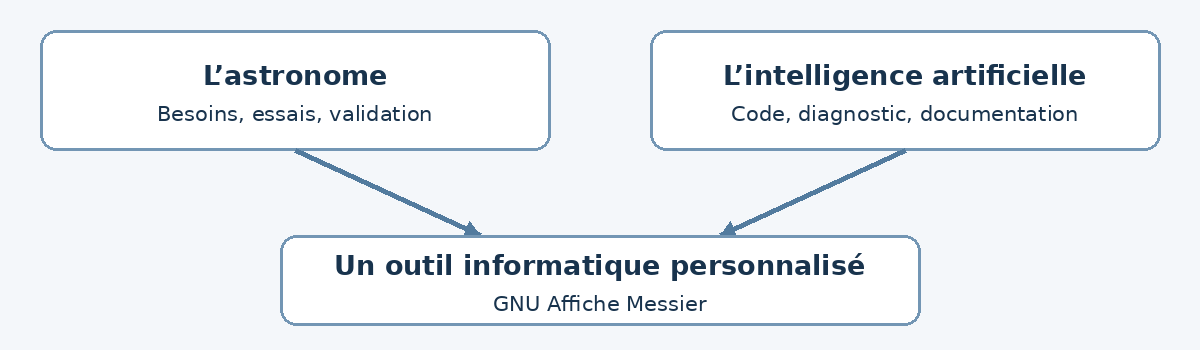
\includegraphics[width=\linewidth,height=40mm,keepaspectratio]{figures/image1.png}\par{\scriptsize Figure 1.1 — Complémentarité entre l'astronome et l'intelligence artificielle (Prud'Homme, 2025).\par}\end{minipage}\par

\par\medskip\repere{Texte oral}

Bonsoir à toutes et à tous. Je suis très heureux de vous retrouver ce soir pour explorer ensemble un sujet qui transforme profondément notre manière d'interagir avec l'informatique, en particulier dans notre passion commune qu'est l'astronomie amateur. Pendant des décennies, si vous aviez une idée de petit logiciel pour gérer vos soirées d'observation, trier vos milliers de photos ou calculer la visibilité d'une comète depuis votre cour arrière, vous faisiez face à un mur : il fallait apprendre un langage de programmation, maîtriser sa syntaxe, installer des environnements complexes et passer des semaines à chasser des erreurs de ponctuation. Aujourd'hui, cette barrière est en train de tomber. Nous allons parler pendant les deux prochaines heures de ce qu'on appelle le Vibe Coding — ou programmation par l'intention en langage naturel —, une approche popularisée par le chercheur Andrej Karpathy (2025a). L'objectif de cette soirée n'est pas de faire de vous des ingénieurs logiciels, mais de vous montrer comment un astronome amateur, sans formation en programmation, peut dialoguer avec une intelligence artificielle pour concevoir, tester, documenter et partager de véritables logiciels libres. Nous verrons les forces et les pièges de cette méthode, l'art de rédiger de bonnes requêtes, les coûts réels, la gestion de versions avec Git et GitHub, et nous plongerons dans quatre projets concrets développés pour mon Seestar S50.\par

\clearpage\repere{DIAPOSITIVE 02 / 45 · 0:02 – 0:05 · 3 min}

{\Large\bfseries Notre parcours, de l'idée au ciel\par}

\smallskip\hrule\smallskip

{\small\textbf{Repère visuel.} Feuille de route chronologique en 8 étapes avec repères horaires (total 120 minutes).\par}

\begin{minipage}[t]{.86\linewidth}\centering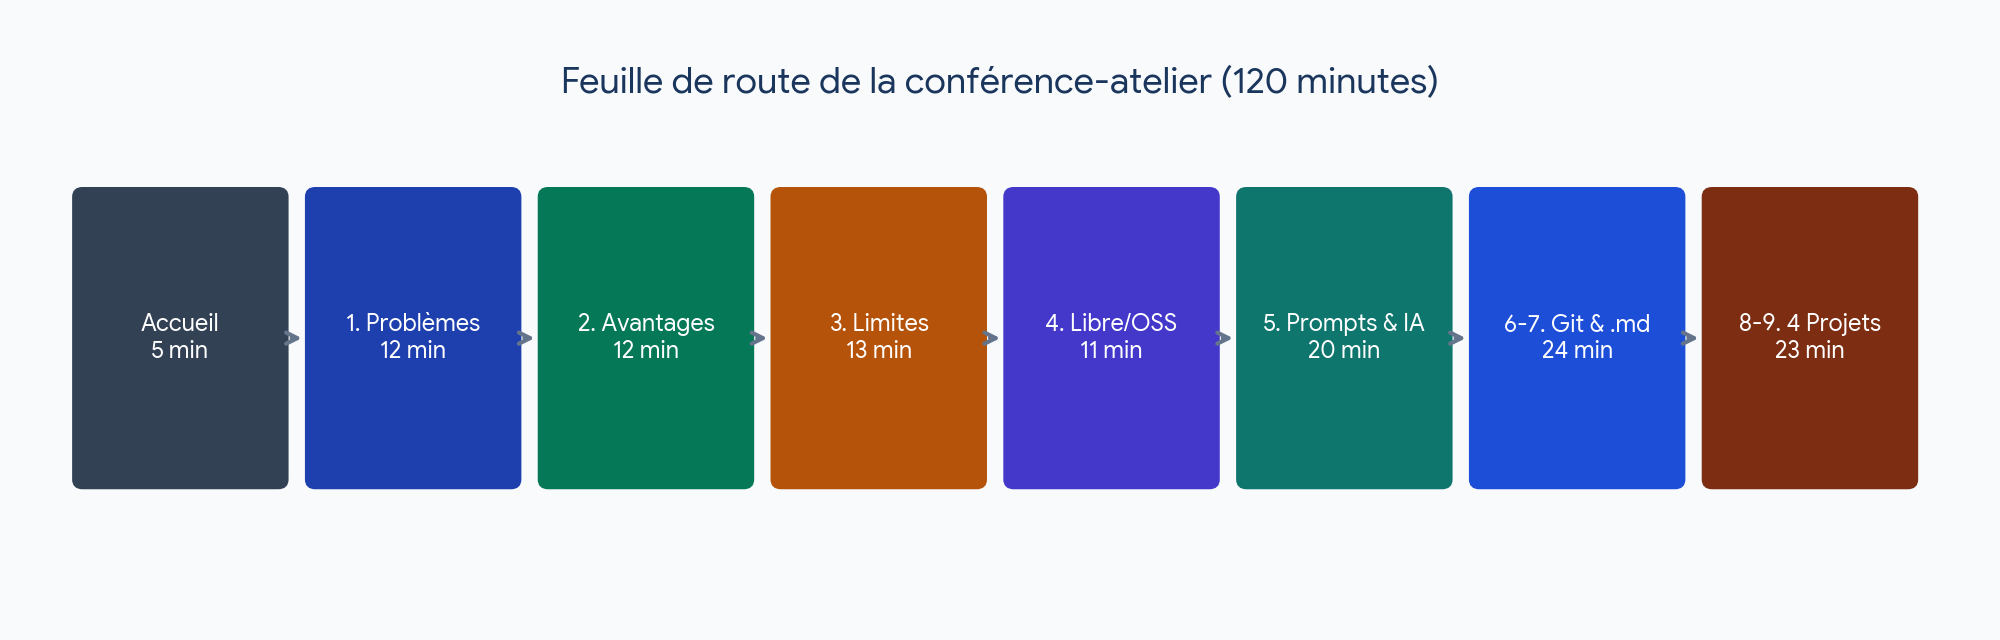
\includegraphics[width=\linewidth,height=40mm,keepaspectratio]{figures/image2.png}\par{\scriptsize Figure 2.1 — Feuille de route chronologique de la conférence-atelier (120 minutes).\par}\end{minipage}\par

\par\medskip\repere{Texte oral}

Voici comment notre soirée est structurée afin que vous repartiez avec une méthode complète et réaliste. Dans un premier temps, nous examinerons quels problèmes concrets l'intelligence artificielle résout pour un non-développeur qui souhaite créer un outil. Ensuite, nous analyserons les cinq grands avantages du Vibe Coding, résumés par l'acronyme anglais FAAFO proposé par Kim et Yegge (2025), mais nous prendrons aussi le temps d'aborder froidement ses désavantages : pourquoi l'IA se trompe, pourquoi elle invente parfois des données astronomiques et comment éviter de se retrouver avec un programme inutilisable. Nous ferons ensuite un détour essentiel par la philosophie du logiciel libre et de l'open source (Meeker, 2020 ; Fogel, 2022), car partager nos outils entre astronomes fait partie intégrante de l'esprit scientifique. Au cœur de la présentation, nous décortiquerons le prompt : qu'est-ce qu'une bonne instruction, quelles sont les meilleures pratiques d'ingénierie de requête (Osmani, 2025 ; Ernaux, 2025), et surtout, comment s'y retrouver entre les différents modes d'un outil comme ChatGPT — les modes Chat, Work et Codex — ainsi que leur consommation en tokens et leur coût réel (OpenAI, 2026a, 2026b). Puis, nous ouvrirons le capot d'un projet libre pour voir comment organiser ses dossiers, quels fichiers Markdown rédiger et comment sécuriser son travail avec Git et GitHub grâce aux commits et au versionnement sémantique. Enfin, dans la dernière portion, je vous présenterai quatre études de cas authentiques issues de ma pratique avec le Seestar S50, incluant mes erreurs de parcours et la première conversation réelle avec ChatGPT qui a lancé le projet GNUAfficheMessier.\par

\clearpage\repere{DIAPOSITIVE 04 / 45 · 0:05 – 0:08 · 3 min}

{\Large\bfseries Décrire le résultat que l'on cherche\par}

\smallskip\hrule\smallskip

{\small\textbf{Repère visuel.} Schéma comparatif « Programmation traditionnelle vs Vibe Coding » adapté de Liew (2026) et Osmani (2025).\par}

\begin{minipage}[t]{.86\linewidth}\centering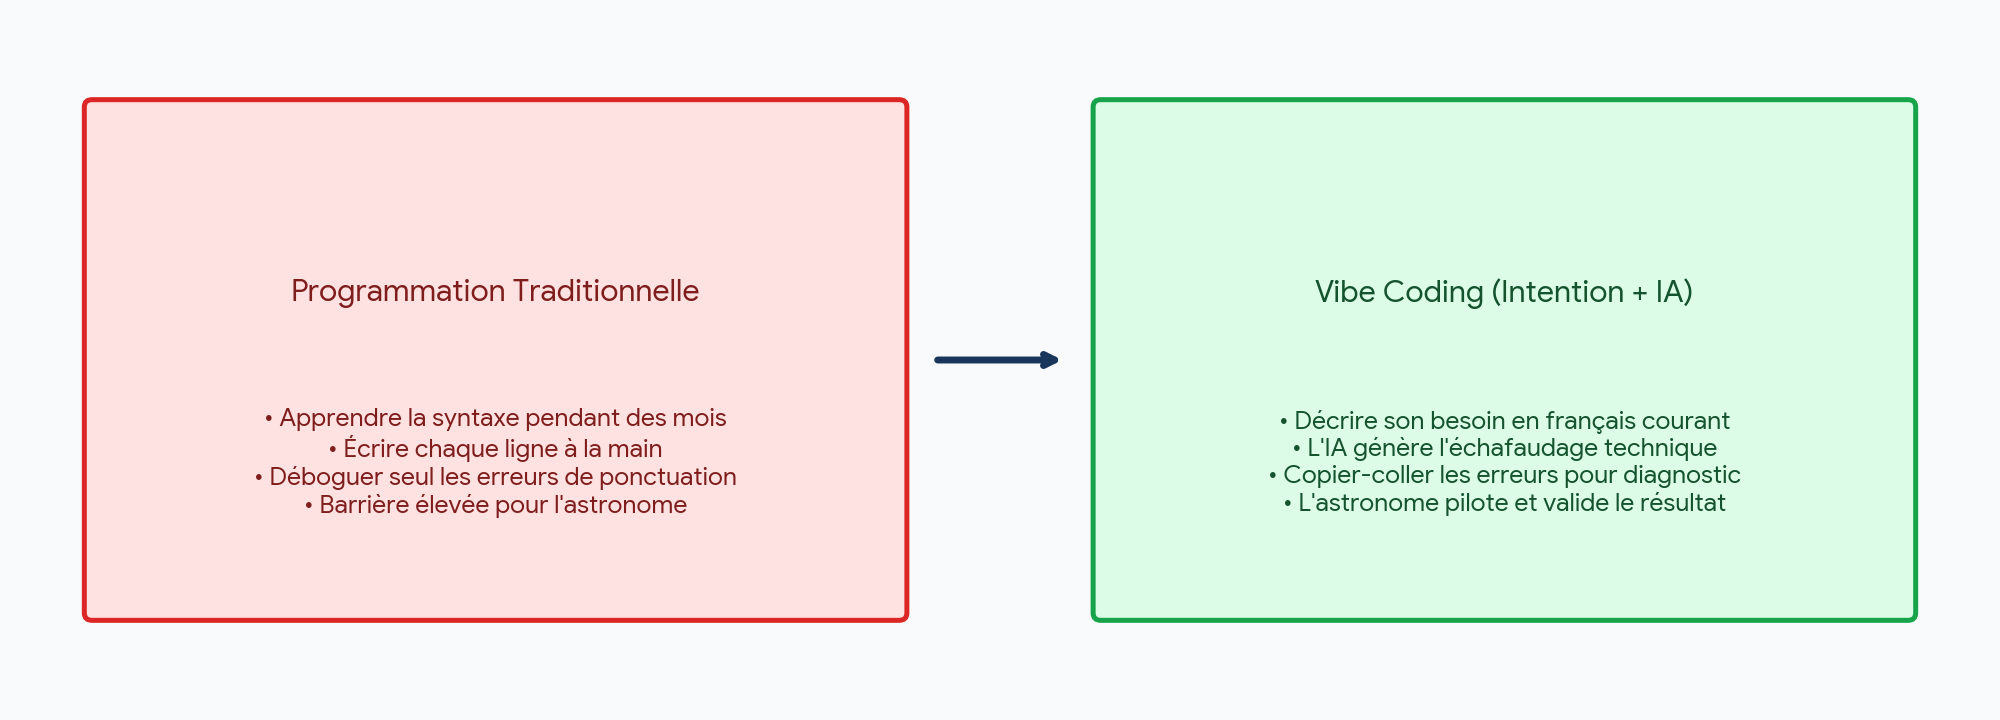
\includegraphics[width=\linewidth,height=40mm,keepaspectratio]{figures/image3.png}\par{\scriptsize Figure 3.1 — Comparaison entre programmation traditionnelle et Vibe Coding.\par}\end{minipage}\par

\par\medskip\repere{Texte oral}

Commençons par la première question : quels sont les problèmes spécifiques que l'intelligence artificielle permet de régler lorsqu'on aborde le développement logiciel ? Le tout premier obstacle, pour un astronome amateur qui n'est pas programmeur, c'est ce que j'appelle le « mur de la syntaxe et de la page blanche ». Comme le soulignent Porter et Zingaro (2024), l'apprentissage traditionnel de la programmation exigeait jadis des mois consacrés à mémoriser des règles grammaticales strictes, à comprendre où placer chaque point-virgule ou chaque indentation, et à installer des bibliothèques logicielles avant même d'afficher un seul mot à l'écran. Une simple faute de frappe bloquait tout le programme. Avec le Vibe Coding, terme inventé par Andrej Karpathy (2025a) pour décrire une approche où l'on « s'abandonne à l'intention » en conversant avec un grand modèle de langage, l'IA prend en charge la traduction mécanique entre votre idée et le code informatique. Vous n'avez plus besoin de connaître par cœur les commandes de la bibliothèque Python Astropy pour lire l'en-tête d'un fichier FITS, ni la syntaxe de ReportLab pour dessiner un tableau dans un fichier PDF (Liew, 2026 ; Prud'Homme, 2025). L'IA agit comme un interprète universel : vous lui décrivez le comportement souhaité en langage courant, et elle génère l'échafaudage technique. Cela résout immédiatement le problème de l'inertie de départ et de la configuration technique qui décourageait la majorité des débutants (Kim et Yegge, 2025).\par

\clearpage\repere{DIAPOSITIVE 05 / 45 · 0:08 – 0:11 · 3 min}

{\Large\bfseries Relier des outils déjà éprouvés\par}

\smallskip\hrule\smallskip

{\small\textbf{Repère visuel.} Schéma d'architecture ECC-G de GNU Astrolist illustrant l'intégration des modules métier et des sorties (Prud'Homme, 2026b).\par}

\begin{minipage}[t]{.86\linewidth}\centering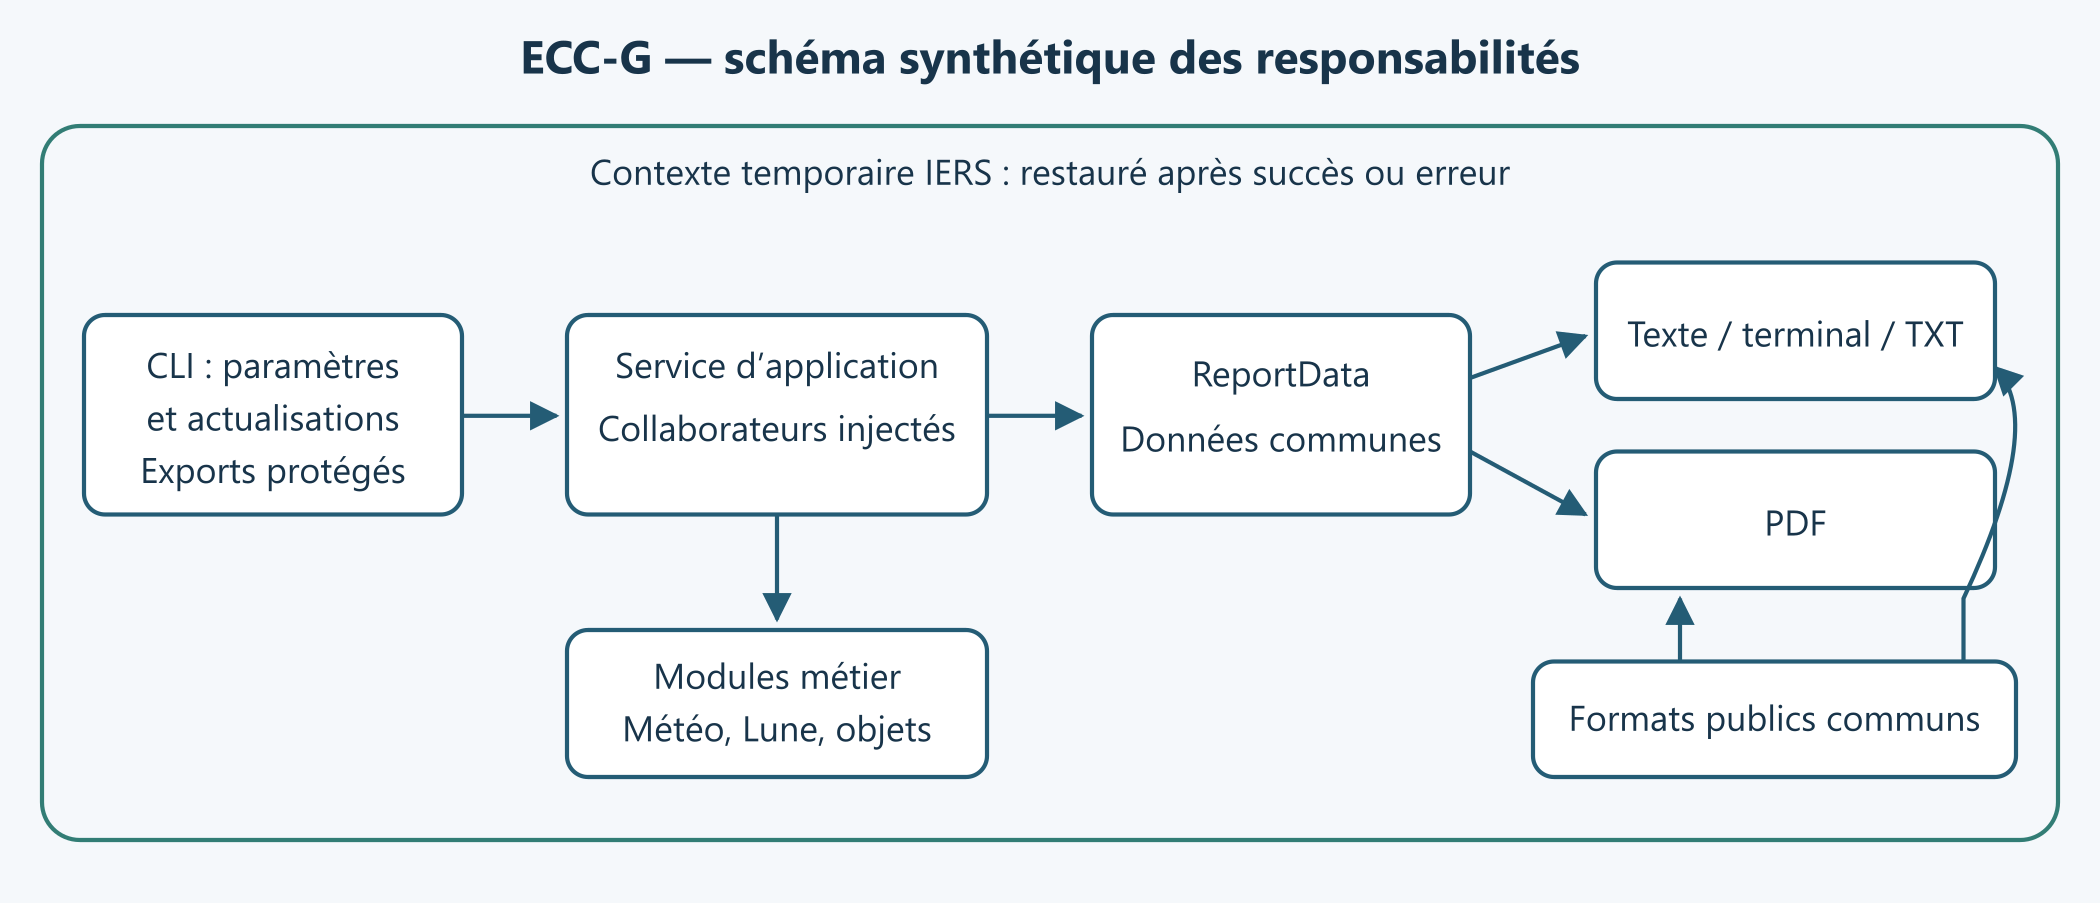
\includegraphics[width=\linewidth,height=40mm,keepaspectratio]{figures/image4.png}\par{\scriptsize Figure 4.1 — Architecture modulaire reliant paramètres, modules métier et sorties multiples (Prud'Homme, 2026b).\par}\end{minipage}\par

\par\medskip\repere{Texte oral}

Le deuxième grand problème résolu par l'IA est celui de l'intégration de technologies hétérogènes. En astronomie amateur, nos besoins sont rarement simples. Prenons un exemple concret : vous voulez créer une page Web pour chacune de vos astrophotographies. Pour y parvenir, votre programme doit lire les métadonnées techniques cachées dans un fichier FITS, interroger la base de données astronomique SIMBAD sur Internet pour obtenir la magnitude et le type de galaxie, calculer les coordonnées astrométriques, récupérer l'historique météo de la nuit d'observation via l'API Open-Meteo, tracer une carte stellaire avec Matplotlib et générer du code HTML propre (Prud'Homme, 2026a). Pour un non-développeur, lire la documentation technique de cinq bibliothèques différentes représente des dizaines d'heures de travail. Or, les grands modèles de langage ont été entraînés sur des millions de dépôts de code public et maîtrisent les interfaces de programmation de la quasi-totalité des outils scientifiques existants (Osmani, 2025). L'IA joue ici le rôle d'un intégrateur système : elle sait comment faire dialoguer ces différentes briques logicielles entre elles et génère le « code de liaison » (glue code) nécessaire pour automatiser des flux de données complexes (Kim et Yegge, 2025 ; Ernaux, 2025).\par

\smallskip\textbf{Animation proposée.} Demandez au groupe de nommer l'information que chaque outil ajoute à une image.

\clearpage\repere{DIAPOSITIVE 06 / 45 · 0:11 – 0:14 · 3 min}

{\Large\bfseries Transformer une erreur en indice\par}

\smallskip\hrule\smallskip

{\small\textbf{Repère visuel.} Tableau des erreurs réelles rencontrées et résolues lors du développement de GNU Affiche Messier (Prud'Homme, 2025).\par}

\begin{minipage}[t]{.86\linewidth}\centering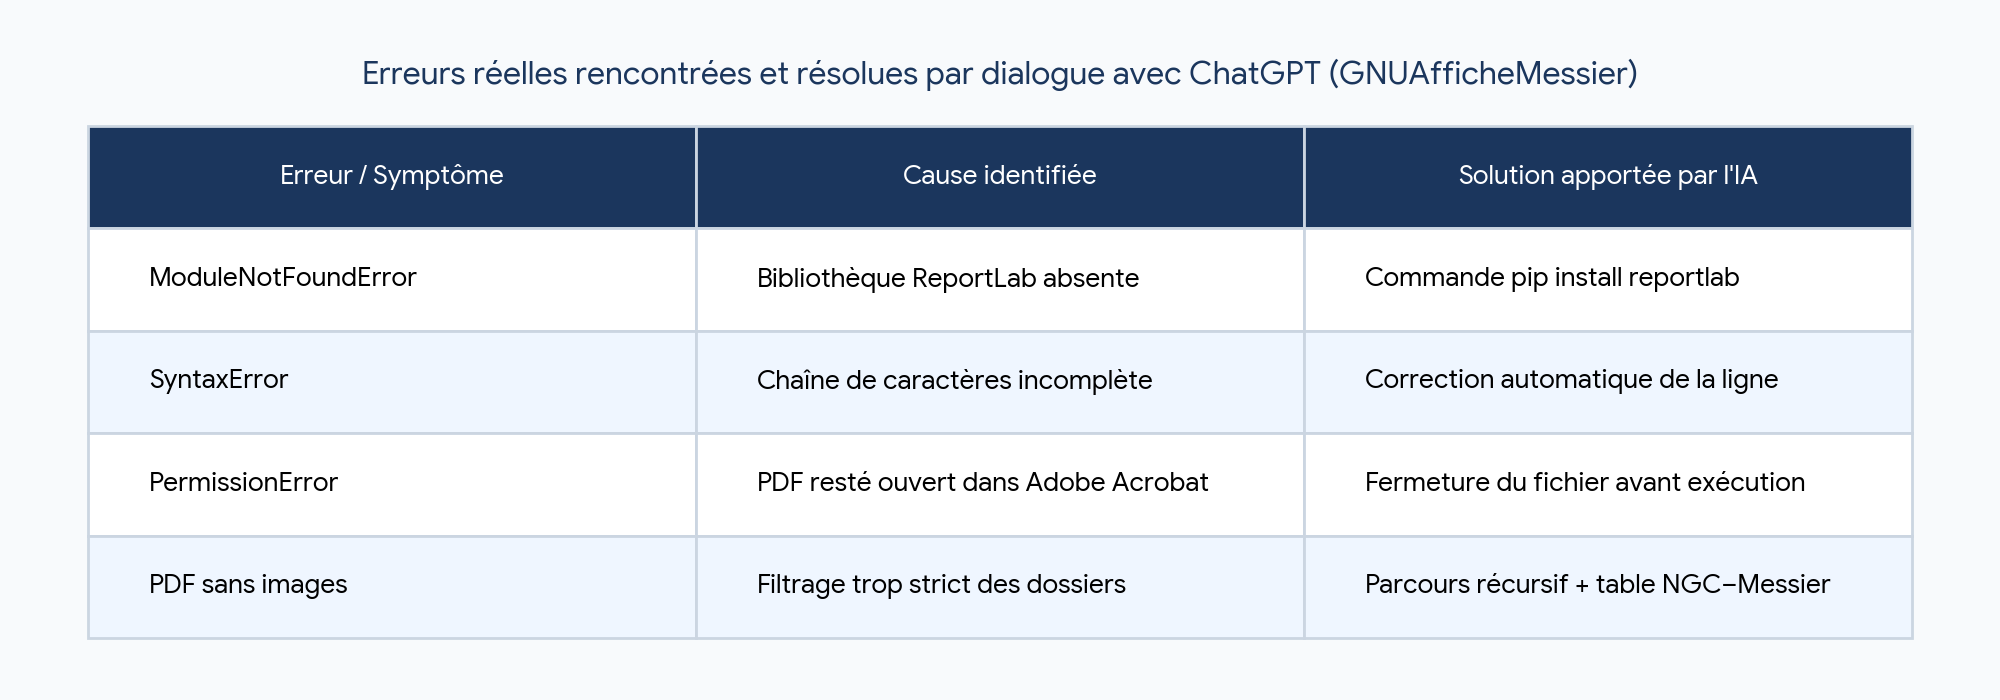
\includegraphics[width=\linewidth,height=40mm,keepaspectratio]{figures/image5.png}\par{\scriptsize Figure 5.1 — Erreurs réelles rencontrées et résolues par dialogue avec ChatGPT (Prud'Homme, 2025).\par}\end{minipage}\par

\par\medskip\repere{Texte oral}

Troisième problème résolu : la paralysie face aux messages d'erreur et la compréhension du code existant. Lorsque vous lancez un script sur votre ordinateur et que le terminal affiche vingt lignes rouges se terminant par ModuleNotFoundError ou PermissionError, un non-développeur se sent immédiatement bloqué. Dans le paradigme du Vibe Coding, le message d'erreur n'est plus une impasse, c'est un indice que vous transmettez directement à votre assistant (Kim et Yegge, 2025 ; Liew, 2026). Par exemple, lors de la création de GNU Affiche Messier, mon programme a planté avec une erreur d'autorisation d'écriture. J'ai simplement copié l'erreur dans ChatGPT, qui m'a fait remarquer que le fichier PDF était resté ouvert dans Adobe Acrobat sur mon écran, empêchant Python de le remplacer (Prud'Homme, 2025). De plus, l'IA résout le problème de la « boîte noire » : vous pouvez lui demander à tout moment d'expliquer une fonction ligne par ligne avec des métaphores simples, comme le recommande Ernaux (2025), ou de reprendre un vieux projet abandonné depuis des années pour en cartographier la structure (Prud'Homme, 2026b).\par

\clearpage\repere{DIAPOSITIVE 07 / 45 · 0:14 – 0:17 · 3 min}

{\Large\bfseries Automatiser une tâche répétitive\par}

\smallskip\hrule\smallskip

{\small\textbf{Repère visuel.} Graphique comparatif entre le travail manuel théorique (24 h 30 pour 147 photos) et l'exécution automatisée en une commande.\par}

\begin{minipage}[t]{.86\linewidth}\centering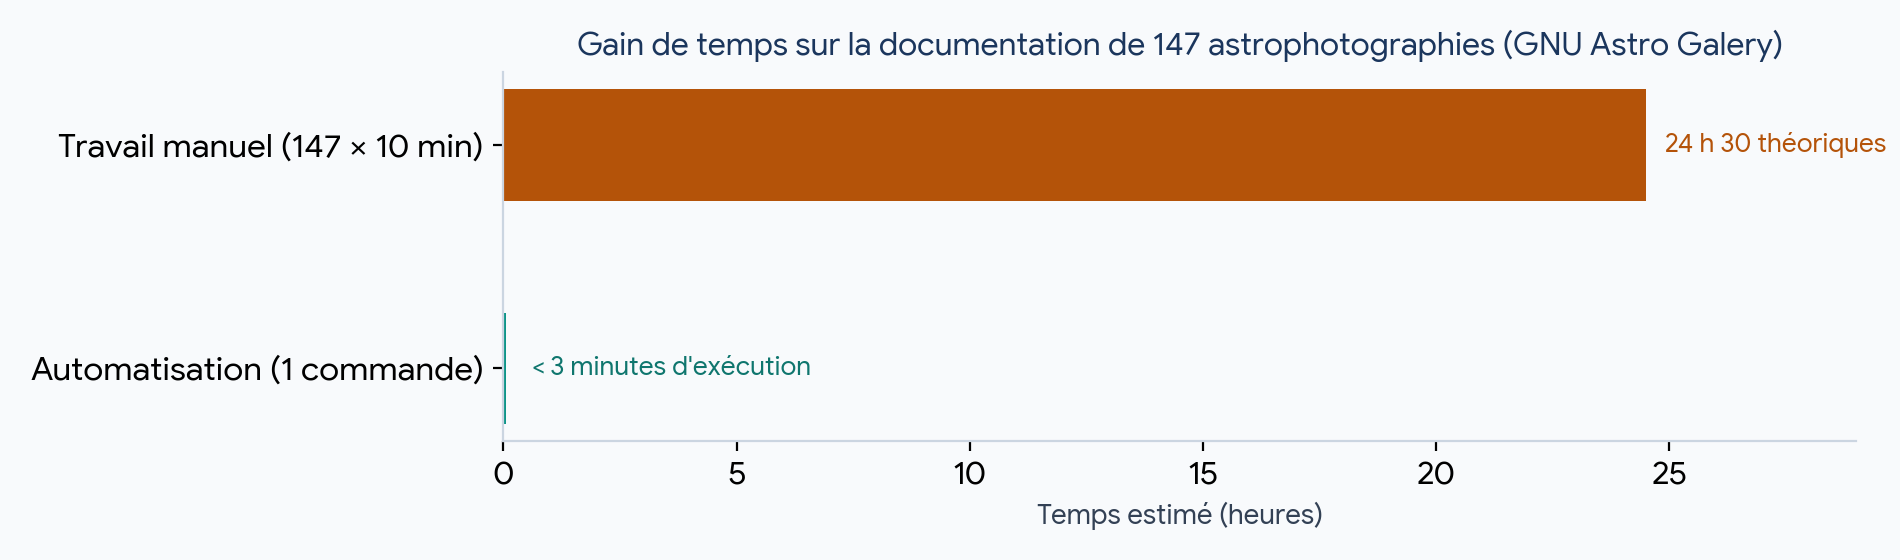
\includegraphics[width=\linewidth,height=40mm,keepaspectratio]{figures/image6.png}\par{\scriptsize Figure 6.1 — Gain de temps estimé sur la documentation de 147 astrophotographies (Prud'Homme, 2026a).\par}\end{minipage}\par

\par\medskip\repere{Texte oral}

Enfin, le quatrième problème que l'IA résout est d'ordre économique et pratique : la création d'outils de niche hyper-spécialisés. Les éditeurs de logiciels commerciaux développent des produits pour le plus grand nombre, jamais pour le flux de travail très particulier d'un astronome qui possède un Seestar S50, qui observe depuis un balcon orienté sud-ouest et qui souhaite générer une affiche murale de 24 par 36 pouces en français (Prud'Homme, 2025, 2026b). Auparavant, le retour sur investissement d'un tel petit programme était trop faible pour justifier d'engager un développeur ou d'apprendre à coder pendant six mois. Comme le soulignent Kim et Yegge (2025), le Vibe Coding élargit les deux extrémités du spectre des projets réalisables : il rend accessibles des projets ambitieux, tout en rendant rentables de petits utilitaires personnels qui éliminent les corvées répétitives. Au lieu de passer vingt-quatre heures à créer manuellement des pages Web pour 147 photographies ou à fouiller dans 18 024 fichiers JPEG, vous créez un script sur mesure en une journée (Prud'Homme, 2025, 2026a).\par

\smallskip\textbf{Animation proposée.} Faites estimer le temps pour dix images puis pour 147. Comparez les hypothèses.

\clearpage\repere{DIAPOSITIVE 09 / 45 · 0:17 – 0:19 · 2 min}

{\Large\bfseries Cinq raisons d'essayer le vibe coding\par}

\smallskip\hrule\smallskip

{\small\textbf{Repère visuel.} Diagramme des 5 piliers du modèle FAAFO (Kim et Yegge, 2025).\par}

\begin{minipage}[t]{.86\linewidth}\centering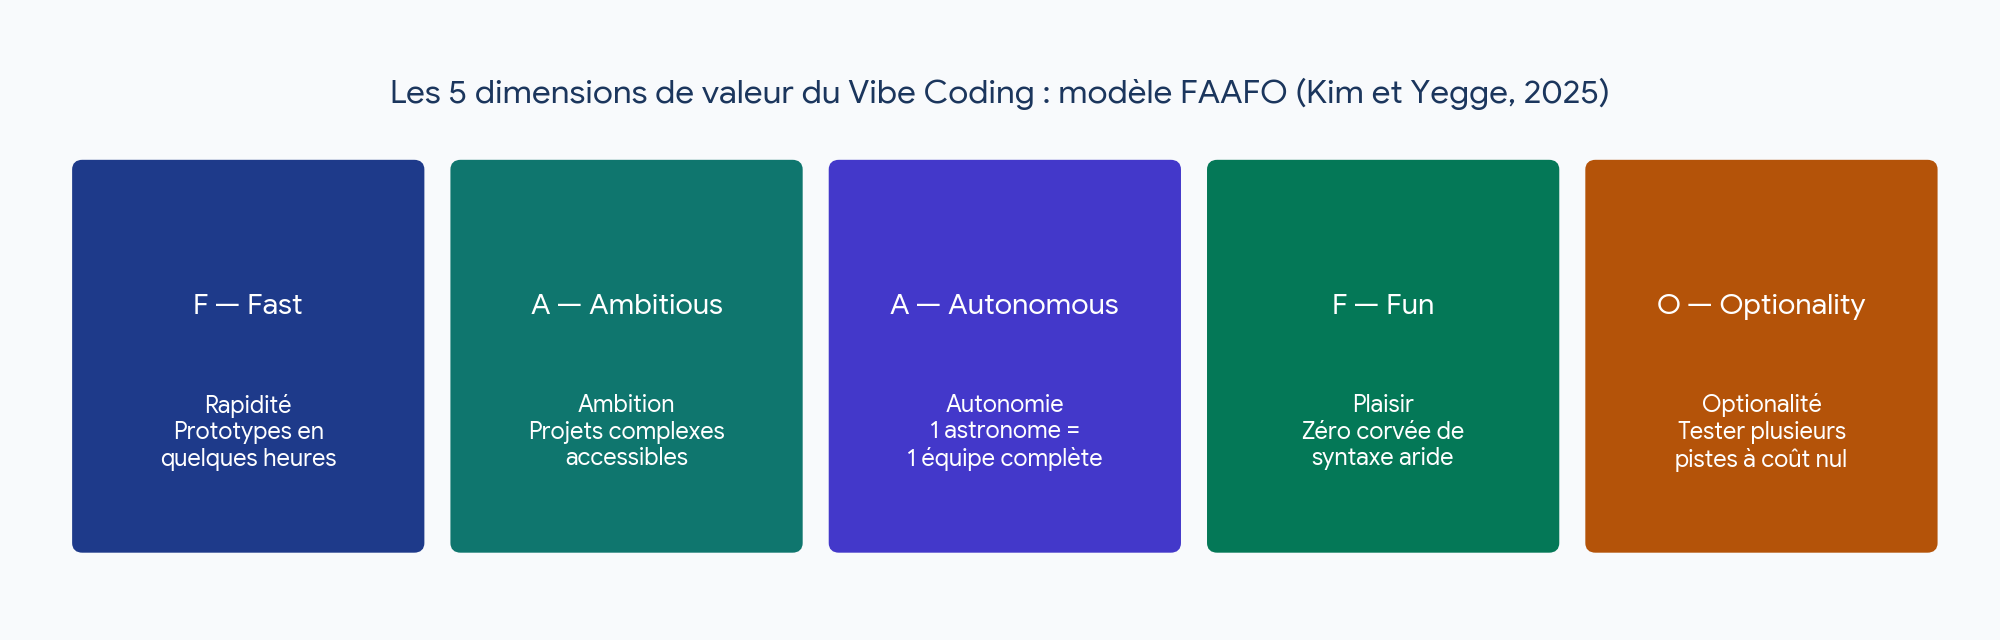
\includegraphics[width=\linewidth,height=40mm,keepaspectratio]{figures/image7.png}\par{\scriptsize Figure 7.1 — Les cinq dimensions de valeur FAAFO du Vibe Coding (Kim et Yegge, 2025).\par}\end{minipage}\par

\par\medskip\repere{Texte oral}

Une fois que l'on comprend quels problèmes l'IA débloque, quels sont les bénéfices concrets que vous allez ressentir en pratiquant le Vibe Coding ? Dans leur ouvrage de référence, Gene Kim et Steve Yegge (2025) synthétisent les avantages de cette approche sous l'acronyme FAAFO, qui désigne cinq dimensions de création de valeur : Fast (la rapidité), Ambitious (l'ambition), Autonomous (l'autonomie), Fun (le plaisir) et Optionality (l'optionalité). Ce cadre est particulièrement éclairant pour nous, astronomes amateurs, car il explique pourquoi des bénévoles ou des passionnés parviennent aujourd'hui à produire des outils qui rivalisent avec des logiciels professionnels. Regardons ces cinq leviers en détail au cours des prochaines diapositives.\par

\clearpage\repere{DIAPOSITIVE 10 / 45 · 0:19 – 0:22 · 3 min}

{\Large\bfseries Passer d'un catalogue à plusieurs\par}

\smallskip\hrule\smallskip

{\small\textbf{Repère visuel.} Schéma de fusion multi-catalogues de GNU Astrolist illustrant l'ambition fonctionnelle (8 317 fiches sources regroupées sans doublon).\par}

\begin{minipage}[t]{.86\linewidth}\centering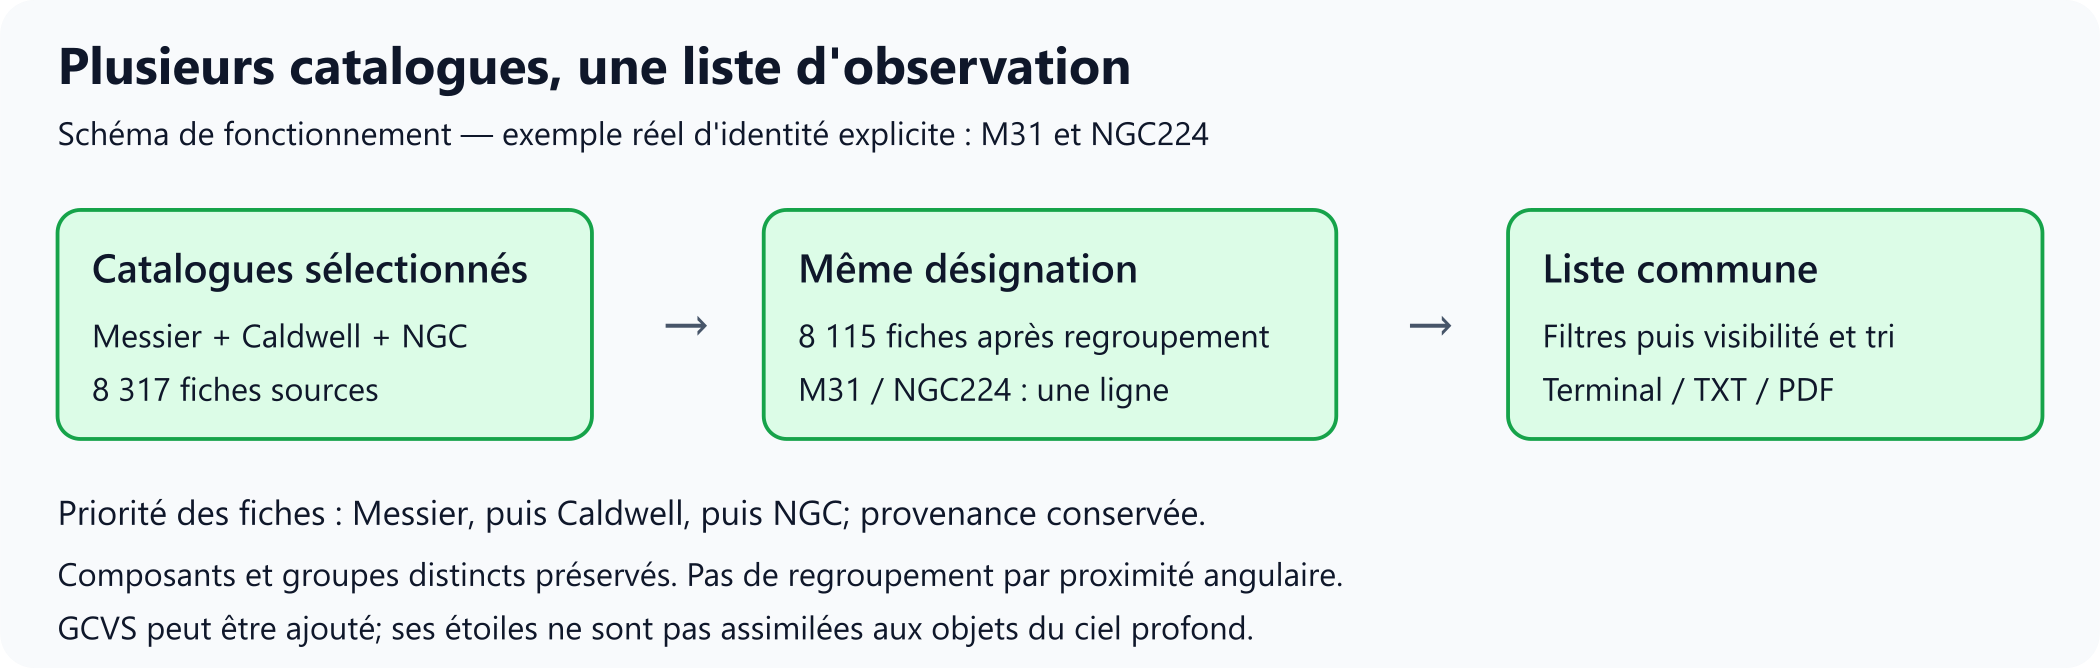
\includegraphics[width=\linewidth,height=40mm,keepaspectratio]{figures/image8.png}\par{\scriptsize Figure 8.1 — Regroupement multi-catalogues Messier, Caldwell et NGC dans GNU Astrolist (Prud'Homme, 2026b).\par}\end{minipage}\par

\par\medskip\repere{Texte oral}

Les deux premiers piliers sont la rapidité (Fast) et l'ambition (Ambitious). Sur le plan de la rapidité, l'accélération ne vient pas uniquement de la génération du code initial, mais aussi de l'aide au débogage, à l'écriture des tests et à la rédaction de la documentation (Kim et Yegge, 2025 ; Liew, 2026). Des études empiriques menées auprès de développeurs montrent d'ailleurs que 84 \% d'entre eux constatent des changements positifs dans leur pratique quotidienne et une réduction marquée du stress lié aux tâches répétitives (Kalliamvakou, 2024). Dans mon propre parcours, le prototype fonctionnel de GNUAfficheMessier a été conçu, testé et documenté au cours d'une seule journée, le 29 décembre 2025 (Prud'Homme, 2025). Cette vitesse nourrit directement le deuxième pilier : l'ambition. Des idées que vous laissiez dormir dans un carnet parce qu'elles semblaient trop complexes deviennent soudainement réalisables. Par exemple, lorsque j'ai repris mon ancien projet GNU Astrolist, je n'ai pas eu à me contenter du seul catalogue Messier : j'ai pu intégrer les catalogues Caldwell et NGC, ajouter le calcul des positions de satellites artificiels, les comètes, les astéroïdes et les phases de la Lune (Prud'Homme, 2026b). L'IA comble nos lacunes techniques et nous permet d'oser des fonctionnalités dignes d'un observatoire.\par

\clearpage\repere{DIAPOSITIVE 11 / 45 · 0:22 – 0:25:30 · 3,5 min}

{\Large\bfseries Garder la main sur son outil\par}

\smallskip\hrule\smallskip

{\small\textbf{Repère visuel.} Schéma illustrant comment un astronome assisté par l'IA remplace une équipe multidisciplinaire.\par}

\begin{minipage}[t]{.86\linewidth}\centering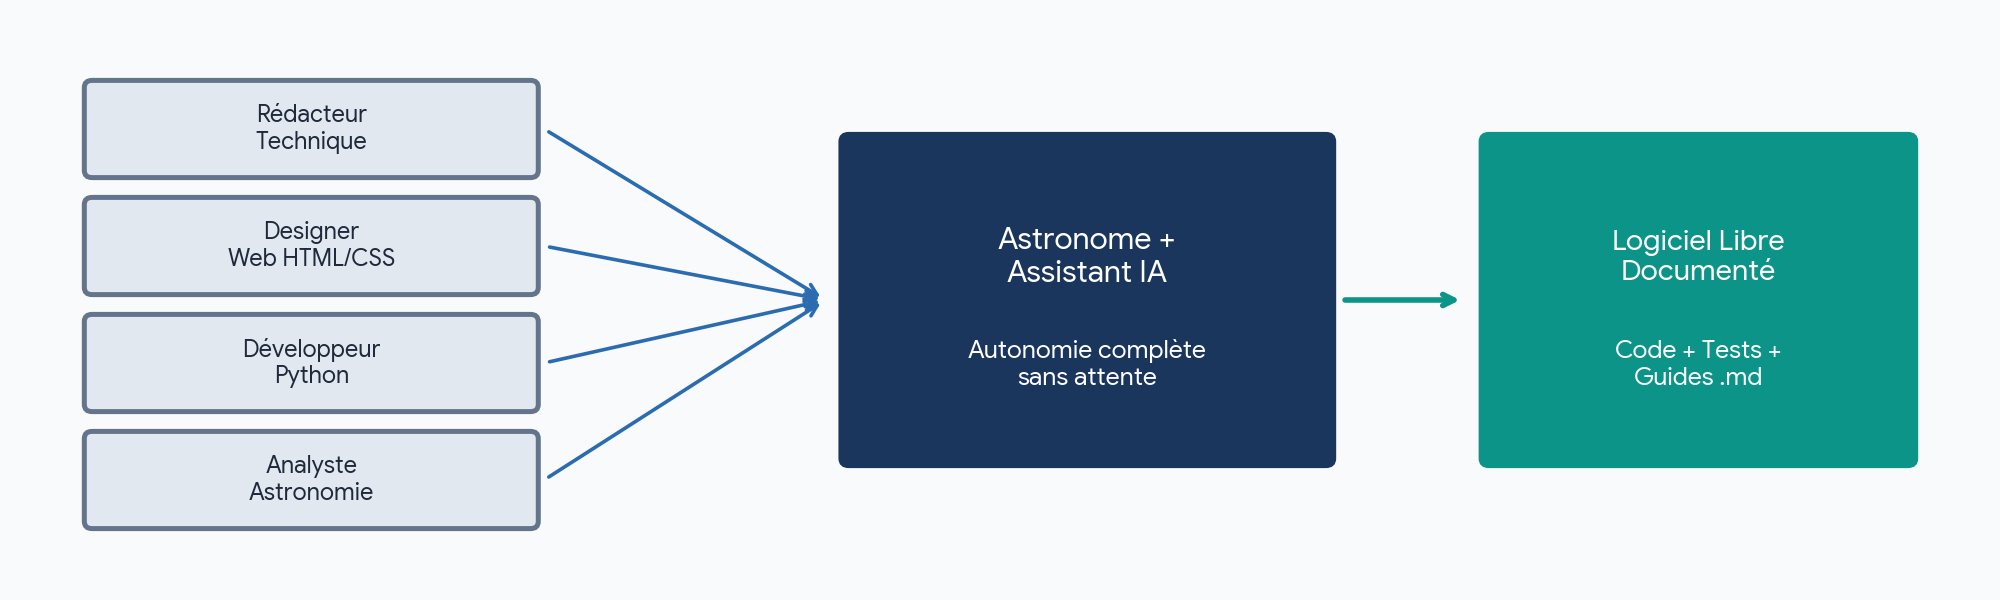
\includegraphics[width=\linewidth,height=40mm,keepaspectratio]{figures/image9.png}\par{\scriptsize Figure 9.1 — Réduction des coûts de coordination grâce à l'autonomie assistée par IA.\par}\end{minipage}\par

\par\medskip\repere{Texte oral}

Les troisième et quatrième avantages sont l'autonomie (Autonomous) et le plaisir (Fun). En informatique traditionnelle, mener à bien un projet complet exige souvent plusieurs spécialistes : un analyste pour les données astronomiques, un développeur backend en Python, un concepteur Web pour le HTML et le CSS, et un rédacteur technique pour le manuel d'utilisation. Coordonner plusieurs personnes engendre des coûts de communication et d'attente énormes (Kim et Yegge, 2025). Grâce à l'IA, un individu seul devient autonome de bout en bout. Vous gardez le contrôle total de votre vision d'astronome tout en déléguant les aspects techniques qui vous échappent. Et cela mène au quatrième avantage, souvent sous-estimé mais fondamental pour un loisir comme l'astronomie : le plaisir (Fun). Comme l'expliquent Kim et Yegge (2025), le Vibe Coding nous épargne les aspects les plus rébarbatifs de la programmation — la configuration des environnements, la lecture de manuels arides, la chasse aux erreurs de syntaxe — pour nous laisser nous concentrer sur la résolution de problèmes concrets et la satisfaction de voir notre outil prendre vie. De plus, c'est un formidable outil d'apprentissage interactif : au lieu de subir un cours magistral abstrait, vous apprenez par la pratique en demandant à l'IA comment fonctionne tel calcul astrométrique ou telle balise FITS (Porter et Zingaro, 2024 ; Ernaux, 2025).\par

\clearpage\repere{DIAPOSITIVE 12 / 45 · 0:25:30 – 0:29 · 3,5 min}

{\Large\bfseries Essayer deux solutions au même besoin\par}

\smallskip\hrule\smallskip

{\small\textbf{Repère visuel.} Schéma du flux automatisé de GNU Astro Galery (Observer \(\rightarrow\) Documenter \(\rightarrow\) Partager sur le Web).\par}

\begin{minipage}[t]{.86\linewidth}\centering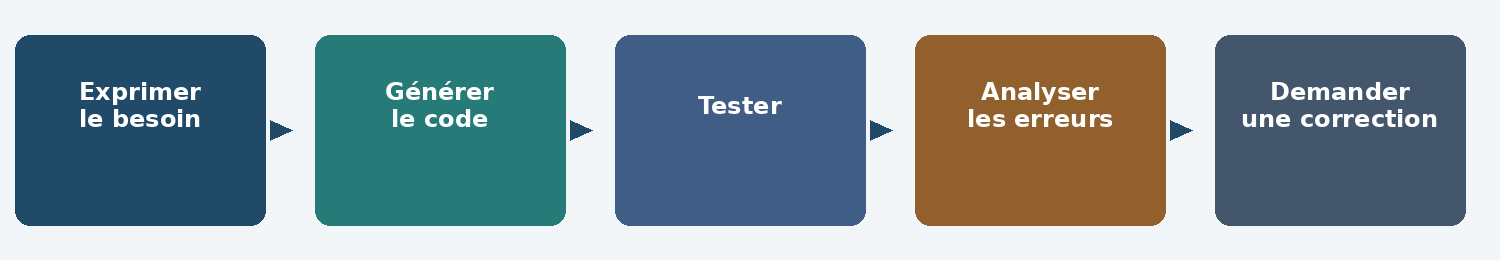
\includegraphics[width=\linewidth,height=40mm,keepaspectratio]{figures/image10.png}\par{\scriptsize Figure 10.1 — Chaîne de traitement automatisée vers le partage Web (Prud'Homme, 2026a).\par}\end{minipage}\par

\par\medskip\repere{Texte oral}

Le cinquième avantage, que Kim et Yegge (2025) considèrent comme le plus profond sur le plan stratégique, est l'optionalité (Optionality). En développement logiciel classique, les premiers choix techniques ressemblent à ce qu'Amazon appelle des « portes à sens unique » : une fois que vous avez écrit deux mille lignes de code pour générer un rapport en format texte, tout convertir en PDF ou en site Web interactif représente un travail colossal, si bien que l'on renonce souvent à explorer d'autres idées. Avec le Vibe Coding, le coût de l'expérimentation chute près de zéro. Vous pouvez demander à votre assistant : « Compare trois façons de générer une carte du ciel en Python : Matplotlib, LaTeX ou SVG, et montre-moi un prototype rapide de la plus simple » (Osmani, 2025 ; Prud'Homme, 2026a). Si une piste ne vous plaît pas, vous la jetez sans regret et vous testez l'alternative en dix minutes. Enfin, un avantage collatéral majeur est la qualité de la documentation : l'IA adore rédiger des fichiers README, des journaux de modifications (Changelog) et des guides d'utilisation clairs, ce qui rend vos outils immédiatement partageables avec les autres membres de votre club d'astronomie (Liew, 2026 ; Prud'Homme, 2025).\par

\clearpage\repere{DIAPOSITIVE 14 / 45 · 0:29 – 0:32:30 · 3,5 min}

{\Large\bfseries Une réponse plausible peut être fausse\par}

\smallskip\hrule\smallskip

{\small\textbf{Repère visuel.} Tableau comparatif des hallucinations astronomiques identifiées dans GNUAfficheMessier.\par}

\begin{minipage}[t]{.86\linewidth}\centering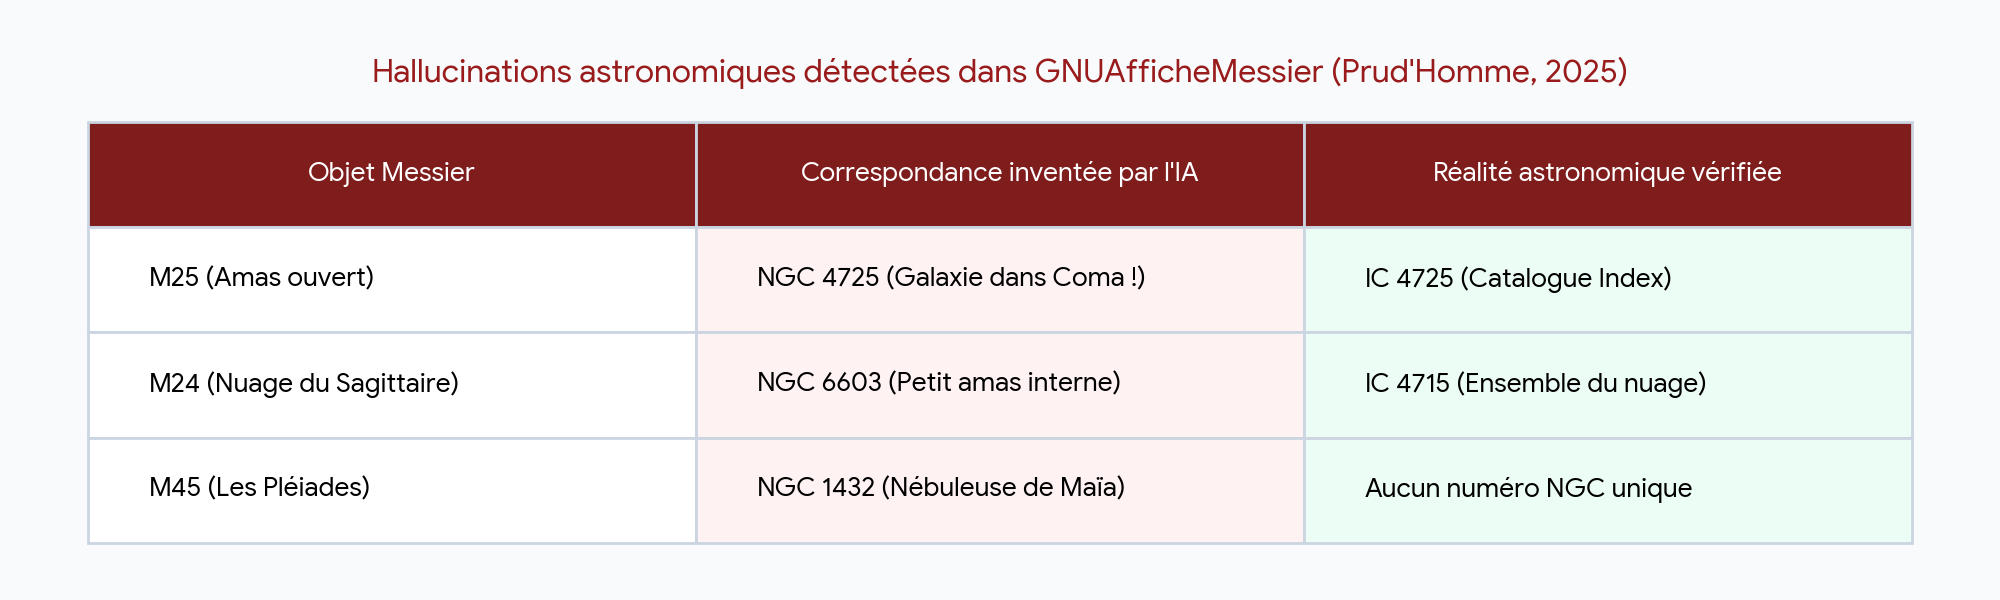
\includegraphics[width=\linewidth,height=40mm,keepaspectratio]{figures/image11.png}\par{\scriptsize Figure 11.1 — Exemples réels d'erreurs scientifiques générées par l'IA (Prud'Homme, 2025).\par}\end{minipage}\par

\par\medskip\repere{Texte oral}

Passons maintenant à l'envers de la médaille. Si le Vibe Coding était magique, nous n'aurions besoin que de dix minutes ce soir. En réalité, utiliser l'IA pour coder comporte des désavantages et des risques majeurs qu'un astronome amateur doit absolument connaître (Osmani, 2025 ; Liew, 2026). Le tout premier danger, c'est ce que j'appelle l'erreur scientifique silencieuse liée aux hallucinations. Comme l'expliquent Martin et Newkirk (2025) ainsi qu'Ernaux (2025), un grand modèle de langage ne « comprend » pas l'univers et ne raisonne pas comme un astrophysicien : il assemble des séquences de texte statistiquement probables avec un ton toujours assuré. Lors du développement de GNUAfficheMessier, j'ai demandé à ChatGPT de générer une table de correspondance entre le catalogue Messier et le catalogue NGC. Le programme tournait sans la moindre erreur informatique ! Pourtant, en vérifiant les résultats avec mes yeux d'astronome, j'ai découvert plusieurs erreurs : pour M25, l'IA avait inventé NGC 4725 au lieu de IC 4725 ; pour M24, elle avait attribué NGC 6603 (qui n'est qu'un petit amas situé à l'intérieur du grand nuage stellaire IC 4715) ; et pour M45, les Pléiades, elle avait assigné NGC 1432, qui n'est qu'une petite nébuleuse autour de l'étoile Maïa (Prud'Homme, 2025). Si vous n'exercez pas votre esprit critique, l'IA inventera des magnitudes ou des coordonnées fausses avec un aplomb total (Prud'Homme, 2026b).\par

\smallskip\textbf{Animation proposée.} Demandez comment vérifier un identifiant douteux. Faites préciser le catalogue et le champ à contrôler.

\clearpage\repere{DIAPOSITIVE 15 / 45 · 0:32:30 – 0:36 · 3,5 min}

{\Large\bfseries Reconnaître une régression\par}

\smallskip\hrule\smallskip

{\small\textbf{Repère visuel.} Graphique en barres horizontales montrant la perte de 30 \% du code (86 Ko \(\rightarrow\) 60 Ko) lors d'une correction sur GNU Astro Galery.\par}

\begin{minipage}[t]{.86\linewidth}\centering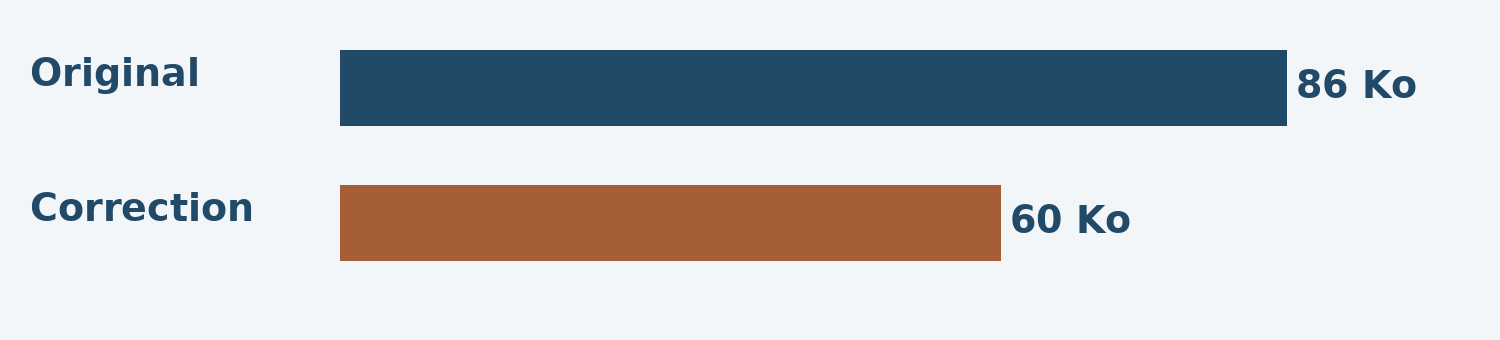
\includegraphics[width=\linewidth,height=40mm,keepaspectratio]{figures/image12.png}\par{\scriptsize Figure 12.1 — Diminution involontaire de 30 \% de la taille du code lors d'une correction IA (Prud'Homme, 2026a).\par}\end{minipage}\par

\par\medskip\repere{Texte oral}

Le deuxième grand désavantage concerne la fragilité du code produit au fil des modifications : les régressions, l'effacement involontaire de fonctions et l'accumulation de dette technique. Kim et Yegge (2025) décrivent avec humour l'IA comme un « sous-chef génial mais imprévisible et bordélique » : un jour elle vous prépare un chef-d'œuvre, le lendemain elle met le feu à la cuisine en détruisant ce qui fonctionnait la veille. Osmani (2025) nomme cela le « problème des 70 \% » : l'IA vous amène très rapidement à 70 \% d'un logiciel fonctionnel, mais dès que vous demandez des ajustements fins, elle risque de casser d'anciennes fonctionnalités. J'en ai fait l'expérience directe sur GNU Astro Galery : à force de demander des ajouts dans un seul gros fichier, le code est devenu si complexe que lors d'une demande de correction, ChatGPT m'a renvoyé un fichier prétendument réparé dont la taille était passée de 86 kilo-octets à 60 kilo-octets ! Il avait silencieusement amputé 30 \% de mon programme (Prud'Homme, 2026a). À un autre moment, coincé dans une boucle de bugs, j'ai même écrit à l'IA : « J'ai l'impression qu'on tourne en rond » (Prud'Homme, 2026a). Sans garde-fous, on se retrouve avec un « château de cartes » numérique impossible à maintenir (Osmani, 2025).\par

\clearpage\repere{DIAPOSITIVE 16 / 45 · 0:36 – 0:39 · 3 min}

{\Large\bfseries Protéger ses fichiers et ses accès\par}

\smallskip\hrule\smallskip

{\small\textbf{Repère visuel.} Schéma du flux de sécurisation : Code généré par IA \(\rightarrow\) Garde-fous (lecture seule) \(\rightarrow\) Validation humaine.\par}

\begin{minipage}[t]{.86\linewidth}\centering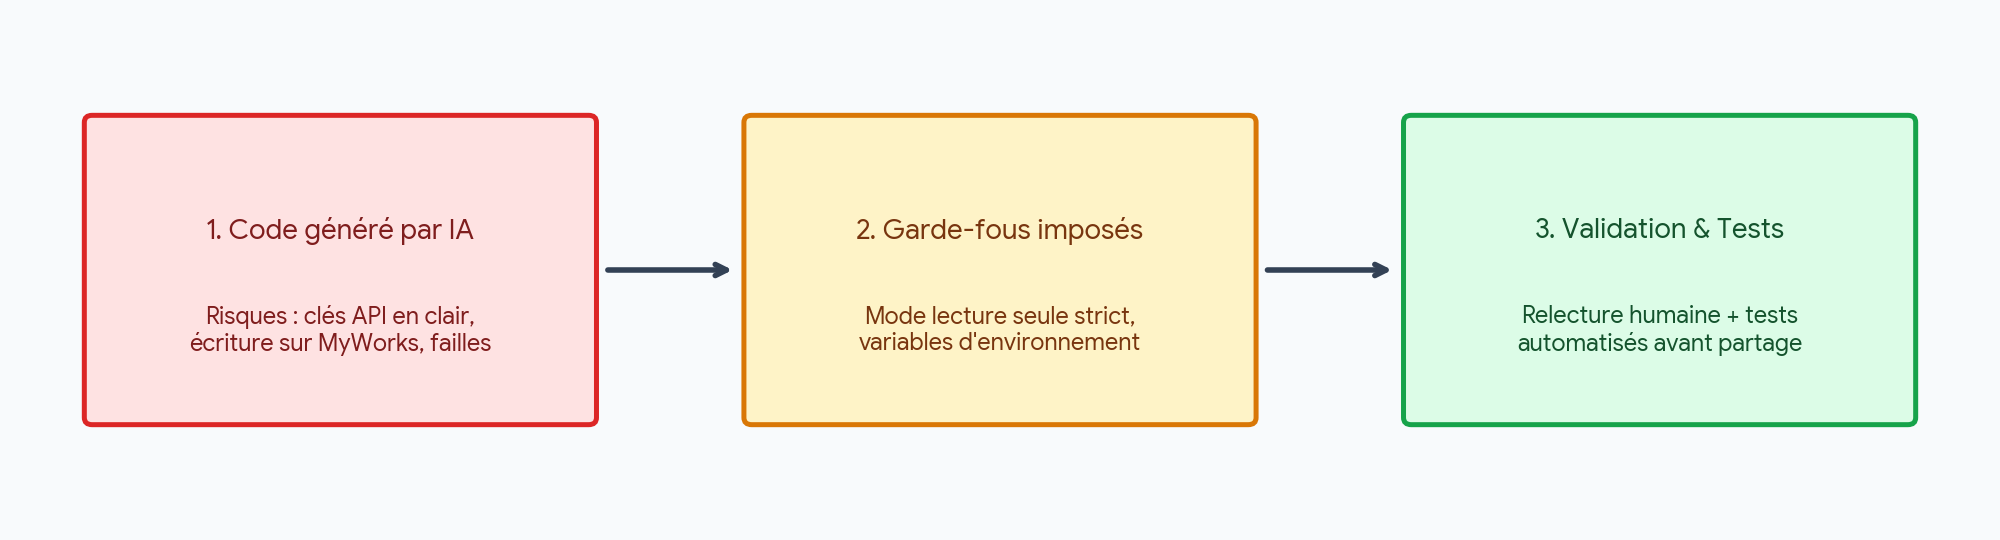
\includegraphics[width=\linewidth,height=40mm,keepaspectratio]{figures/image13.png}\par{\scriptsize Figure 13.1 — Chaîne de prévention des risques de sécurité et de perte de données.\par}\end{minipage}\par

\par\medskip\repere{Texte oral}

Troisième catégorie de désavantages : les risques liés à la sécurité, à l'intégrité de vos données et à la propriété intellectuelle. Comme l'illustre Osmani (2025), les modèles d'IA ont été entraînés sur l'ensemble du Web public, qui contient autant de mauvaises pratiques que de bonnes. Par conséquent, l'IA peut générer du code vulnérable, par exemple en inscrivant en clair une clé d'accès privée dans le script ou en oubliant de vérifier les données saisies par l'utilisateur (Liew, 2026). Pour nous, astronomes amateurs, le risque le plus immédiat est la perte de nos précieuses archives d'observation : si un script mal conçu écrit ou renomme des fichiers directement dans le dossier MyWorks de votre télescope Seestar au lieu de travailler en lecture seule, vous risquez de corrompre vos brutes d'observation (Prud'Homme, 2026b). Par ailleurs, sur le plan de la confidentialité, tout ce que vous copiez dans un assistant infonuagique transite sur des serveurs externes : il ne faut jamais y coller de mots de passe, de clés API ou de données personnelles (Ernaux, 2025). Enfin, sur le plan juridique, le code généré s'inspire de dépôts existants, ce qui soulève des questions de licences logicielles qu'il faut respecter dès que l'on partage son projet (Porter et Zingaro, 2024).\par

\clearpage\repere{DIAPOSITIVE 17 / 45 · 0:39 – 0:42 · 3 min}

{\Large\bfseries Savoir expliquer ce que fait le logiciel\par}

\smallskip\hrule\smallskip

{\small\textbf{Repère visuel.} Schéma du cycle itératif où l'humain reste au centre de l'observation et de la correction.\par}

\begin{minipage}[t]{.86\linewidth}\centering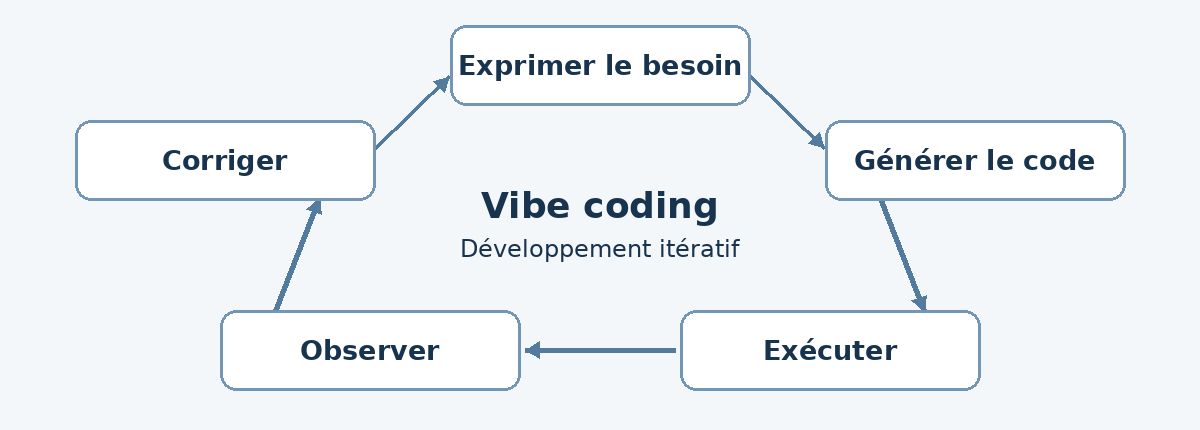
\includegraphics[width=\linewidth,height=40mm,keepaspectratio]{figures/image14.png}\par{\scriptsize Figure 14.1 — Boucle de contrôle humain dans le processus de Vibe Coding (Prud'Homme, 2025).\par}\end{minipage}\par

\par\medskip\repere{Texte oral}

Enfin, le quatrième désavantage est d'ordre cognitif : c'est ce que Porter et Zingaro (2024) appellent le « paradoxe de la connaissance » et ce que Martin et Newkirk (2025) comparent au pilote automatique d'un avion. Un pilote automatique soulage énormément le commandant de bord, mais il ne remplace jamais sa vigilance ni sa compréhension du vol ; si l'automatisme décroche par mauvais temps et que le pilote ne sait plus lire ses instruments, c'est l'accident. En Vibe Coding, si vous cliquez systématiquement sur « Tout accepter » sans chercher à comprendre la logique générale de ce que l'IA construit, vous devenez totalement dépendant d'elle. Dès qu'un bug surviendra, vous serez incapable de lui expliquer où chercher (Osmani, 2025 ; Liew, 2026). La conclusion de cette section est donc claire : l'IA est un stagiaire enthousiaste, doté d'une mémoire encyclopédique mais dépourvu de bon sens astronomique. Vous demeurez le directeur de projet et l'observateur responsable (Liew, 2026 ; Prud'Homme, 2025).\par

\clearpage\repere{DIAPOSITIVE 19 / 45 · 0:42 – 0:45 · 3 min}

{\Large\bfseries Partager le code et les décisions\par}

\smallskip\hrule\smallskip

{\small\textbf{Repère visuel.} Schéma comparatif : Modèle propriétaire fermé (« La Cathédrale ») vs Modèle libre collaboratif (« Le Bazar »).\par}

\begin{minipage}[t]{.86\linewidth}\centering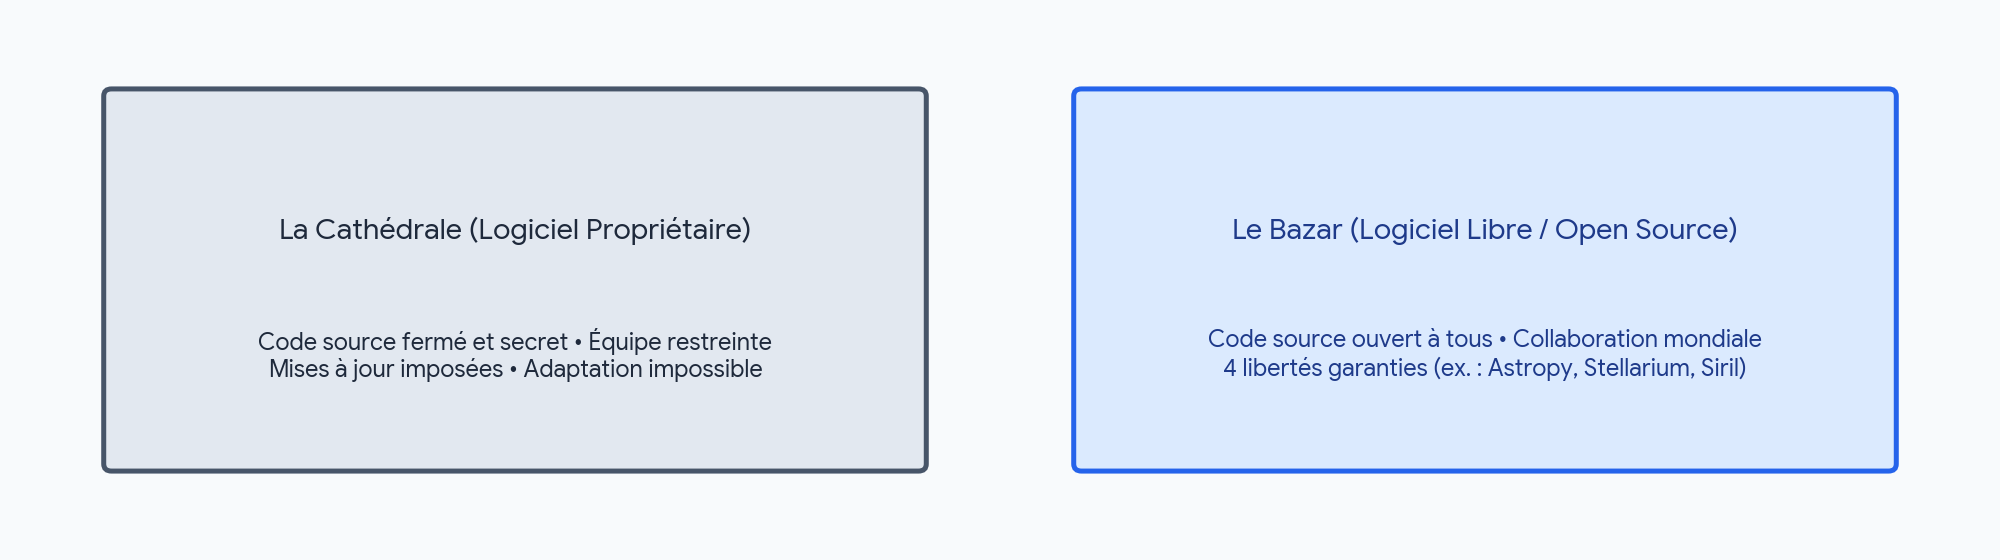
\includegraphics[width=\linewidth,height=40mm,keepaspectratio]{figures/image15.png}\par{\scriptsize Figure 15.1 — Deux philosophies de développement : La Cathédrale vs Le Bazar.\par}\end{minipage}\par

\par\medskip\repere{Texte oral}

Pourquoi tous mes projets d'astronomie commencent-ils par le préfixe « GNU » et sont-ils publiés sous licence libre ? Parce que le Vibe Coding prend tout son sens lorsqu'il s'inscrit dans la culture du logiciel libre et de l'open source. Clarifions d'abord ces deux expressions souvent confondues. Comme l'expliquent Heather Meeker (2020) et Karl Fogel (2022), le mouvement du logiciel libre (Free Software), fondé par Richard Stallman dans les années 1980 avec le projet GNU, repose sur une philosophie éthique : l'utilisateur doit avoir le contrôle sur les outils informatiques qu'il utilise. En anglais, free signifie « libre » (comme dans liberté d'expression) et non pas nécessairement « gratuit » (comme une bière gratuite). À la fin des années 1990, l'Open Source Initiative a proposé le terme Open Source pour mettre l'accent sur l'efficacité pragmatique et collaborative de ce modèle auprès des entreprises et des scientifiques (Eghbal, 2020). Eric Raymond a illustré cette différence par une métaphore célèbre : le logiciel propriétaire est construit comme une cathédrale médiévale, par une équipe fermée derrière des murs ; le logiciel libre se développe comme un bazar ouvert, où chacun peut inspecter les plans, proposer des améliorations et partager ses découvertes (Meeker, 2020).\par

\clearpage\repere{DIAPOSITIVE 20 / 45 · 0:45 – 0:48 · 3 min}

{\Large\bfseries Les quatre libertés d'un club\par}

\smallskip\hrule\smallskip

{\small\textbf{Repère visuel.} Les quatre libertés fondamentales du logiciel libre appliquées à la communauté astronomique.\par}

\par\medskip\repere{Texte oral}

Concrètement, qu'est-ce qui garantit qu'un logiciel est véritablement libre ? La Free Software Foundation définit quatre libertés essentielles, numérotées de 0 à 3 (Meeker, 2020). La Liberté 0 est le droit d'exécuter le programme pour n'importe quel usage, sans limite de temps, de lieu ou de nombre d'ordinateurs. La Liberté 1 est le droit d'étudier comment le programme fonctionne et de l'adapter à vos propres besoins — ce qui exige que le code source (le texte lisible du programme) soit fourni. La Liberté 2 est le droit de redistribuer des copies exactes pour aider vos collègues astronomes. Enfin, la Liberté 3 est le droit d'améliorer le programme et de publier vos modifications pour que toute la communauté en bénéficie. Pensez à ce que cela signifie pour notre club d'astronomie : si je crée un script qui génère une affiche Messier ou une liste d'observation, vous pouvez le télécharger gratuitement, l'ouvrir dans votre éditeur, demander à ChatGPT de l'adapter pour votre télescope Unistellar ou votre monture équatoriale, et partager cette nouvelle version avec le reste du club ! C'est exactement ainsi que fonctionnent des piliers de l'astronomie moderne comme Astropy, Stellarium ou Siril (Eghbal, 2020).\par

\smallskip\textbf{Animation proposée.} Proposez au club de modifier puis de redistribuer un outil. Faites retrouver les libertés mobilisées.

\clearpage\repere{DIAPOSITIVE 21 / 45 · 0:48 – 0:51 · 3 min}

{\Large\bfseries Choisir les conditions de réutilisation\par}

\smallskip\hrule\smallskip

{\small\textbf{Repère visuel.} Comparaison entre licences permissives (MIT/Apache) et licences Copyleft (GNU GPL v3).\par}

\begin{minipage}[t]{.86\linewidth}\centering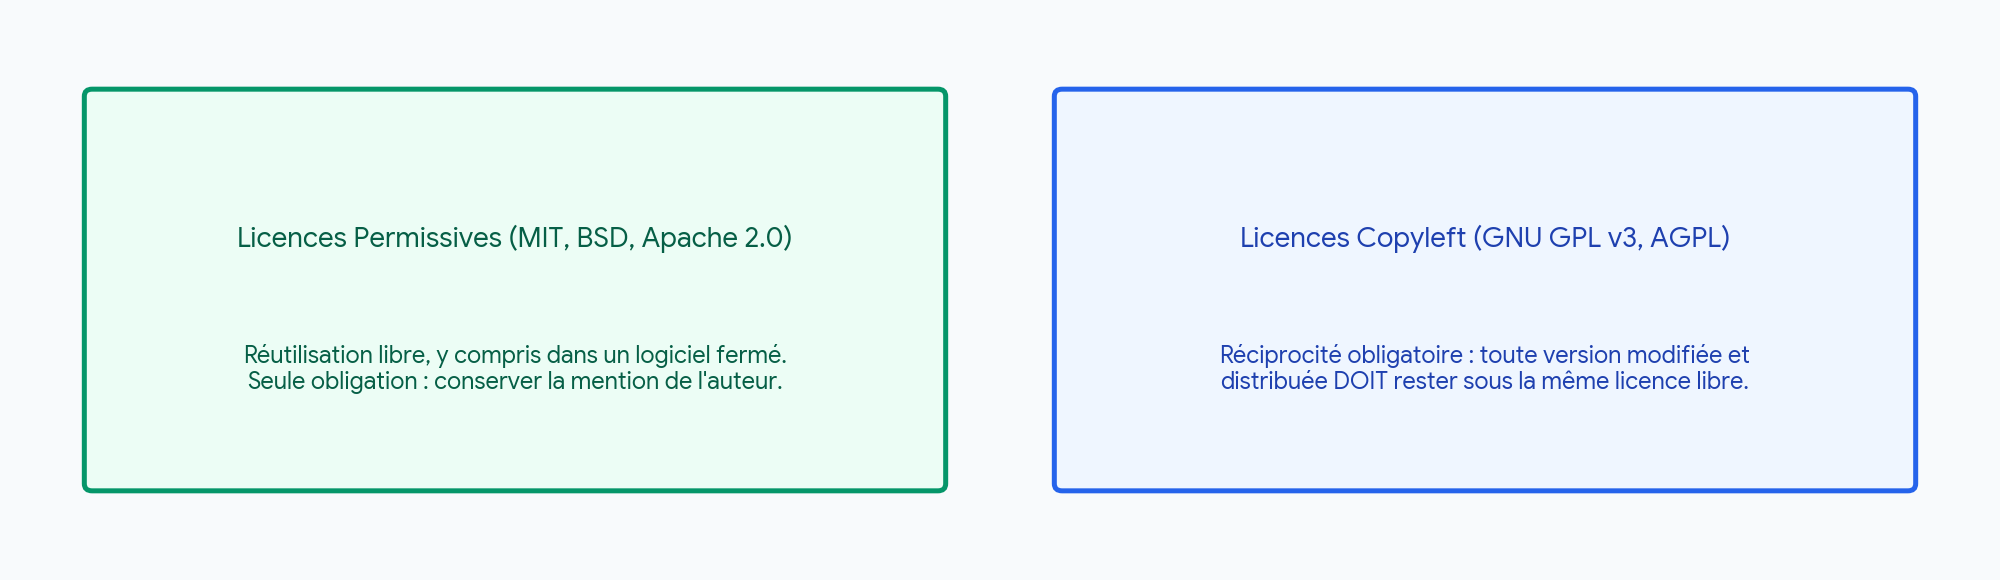
\includegraphics[width=\linewidth,height=40mm,keepaspectratio]{figures/image16.png}\par{\scriptsize Figure 17.1 — Licences permissives vs licences Copyleft (Meeker, 2020 ; Fogel, 2022).\par}\end{minipage}\par

\par\medskip\repere{Texte oral}

Attention toutefois à une idée reçue très fréquente : « open source » ne signifie pas « sans droit d'auteur » ou « domaine public » (Osmani, 2025 ; Meeker, 2020). Par défaut, tout code écrit par un humain est protégé par le droit d'auteur. Une licence libre est une autorisation juridique conditionnelle qui accorde les quatre libertés que nous venons de voir, à condition de respecter certaines règles. On distingue deux grandes familles de licences (Meeker, 2020 ; Fogel, 2022). D'un côté, les licences permissives, comme la licence MIT ou Apache 2.0, qui disent en substance : « Prenez ce code, modifiez-le, intégrez-le même dans un logiciel fermé si vous le souhaitez, à la seule condition de conserver mon nom et la mention de droit d'auteur. » De l'autre côté, les licences Copyleft — dont la plus célèbre est la GNU GPL v3 (General Public License), que j'utilise pour mes projets — imposent une règle de réciprocité : si vous modifiez mon logiciel et que vous le distribuez à d'autres personnes, vous avez l'obligation de fournir le code source modifié sous la même licence GPL. Cela garantit que l'outil restera libre à jamais et ne pourra pas être verrouillé par un acteur commercial. Pour les photographies et documents non logiciels, on utilise plutôt les licences Creative Commons, comme le CC0 (domaine public) que j'applique à mes photos dans Astro Galery (Prud'Homme, 2026a).\par

\clearpage\repere{DIAPOSITIVE 22 / 45 · 0:51 – 0:53 · 2 min}

{\Large\bfseries Qui fait vivre un projet libre?\par}

\smallskip\hrule\smallskip

{\small\textbf{Repère visuel.} Matrice 2\(\times\)2 « Croissance des utilisateurs vs Croissance des contributeurs » d'après Nadia Eghbal (2020, p. 81).\par}

\begin{minipage}[t]{.86\linewidth}\centering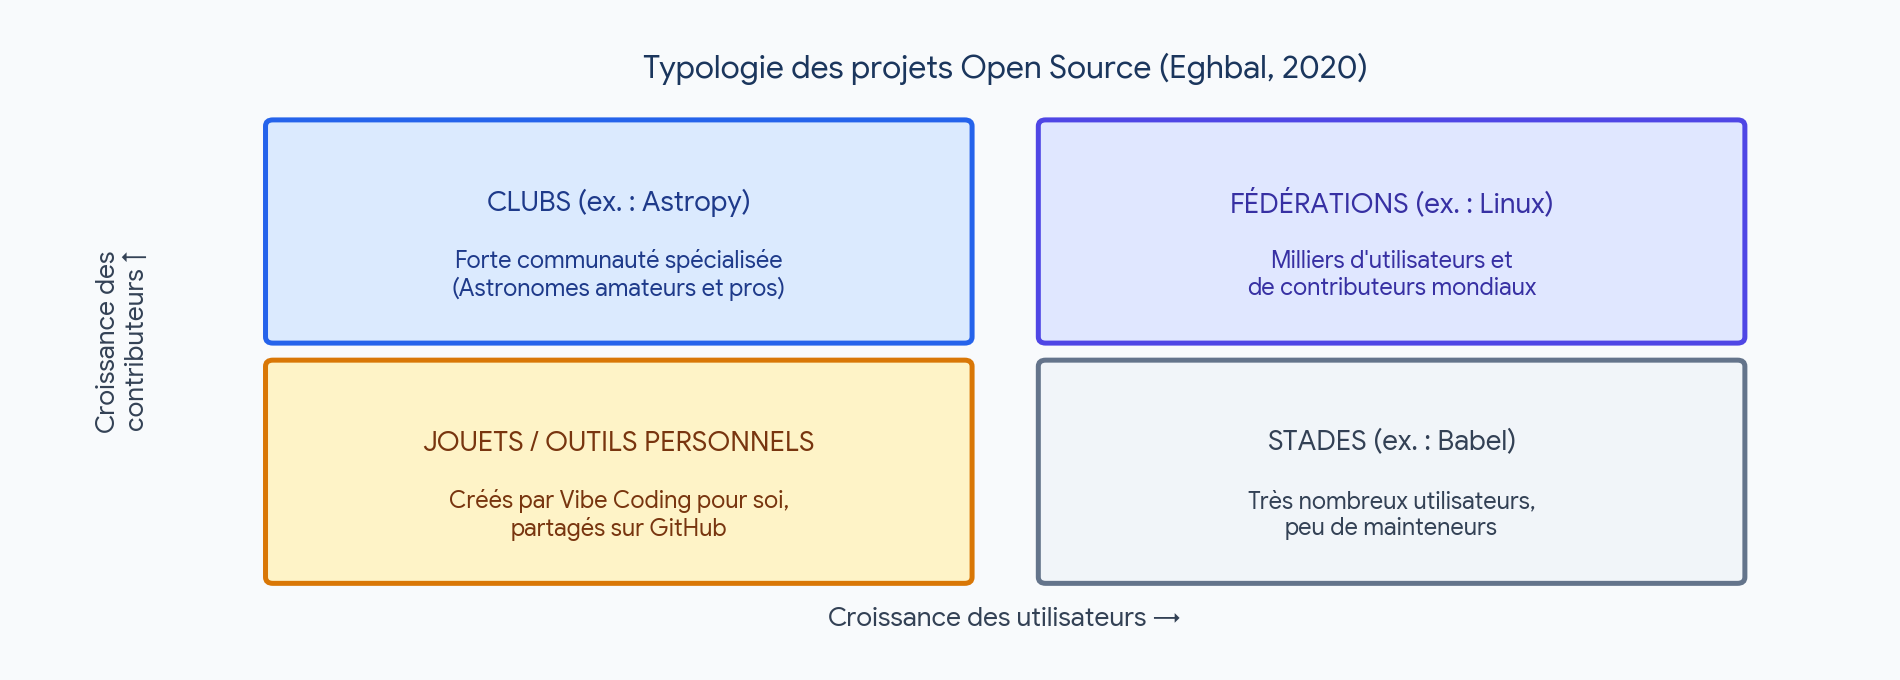
\includegraphics[width=\linewidth,height=40mm,keepaspectratio]{figures/image17.png}\par{\scriptsize Figure 18.1 — Typologie des projets Open Source et positionnement d'Astropy (Eghbal, 2020).\par}\end{minipage}\par

\par\medskip\repere{Texte oral}

Dans son livre Working in Public, la chercheuse Nadia Eghbal (2020) propose une classification fascinante des projets open source selon le nombre d'utilisateurs et de contributeurs. Elle distingue quatre modèles : les Fédérations géantes comme Linux, les Stades, les Clubs — et devinez quel exemple exact elle cite dans son livre pour illustrer un « Club » ? Astropy, la grande bibliothèque Python utilisée par les astronomes professionnels et amateurs du monde entier ! Enfin, la quatrième catégorie est celle des Toys ou outils personnels : de petits logiciels créés au départ pour résoudre le problème d'une seule personne, mais publiés ouvertement sur GitHub. Grâce au Vibe Coding, n'importe quel membre de notre société d'astronomie peut aujourd'hui créer son propre outil personnel et, qui sait, le voir évoluer vers un véritable projet de club !\par

\clearpage\repere{DIAPOSITIVE 24 / 45 · 0:53 – 0:55:30 · 2,5 min}

{\Large\bfseries Un prompt est une consigne\par}

\smallskip\hrule\smallskip

{\small\textbf{Repère visuel.} Schéma du cycle itératif d'affinement des prompts : Exprimer le besoin \(\rightarrow\) Générer \(\rightarrow\) Tester \(\rightarrow\) Analyser \(\rightarrow\) Corriger (Prud'Homme, 2026a).\par}

\textbf{Schéma projeté.} Formulez la demande. Précisez un critère observable. Vérifiez le résultat obtenu avant de poursuivre.\par

\par\medskip\repere{Texte oral}

Nous arrivons maintenant au cœur pratique de notre atelier : le prompt. Qu'est-ce qu'un prompt (ou une invite) ? Comme le définissent Osmani (2025) et Ernaux (2025), un prompt est l'instruction, la question ou la description que vous fournissez à une intelligence artificielle pour qu'elle accomplisse une tâche. En Vibe Coding, le prompt remplace le code source traditionnel comme point de départ : c'est le pont entre votre intention d'astronome et le programme que l'ordinateur va exécuter (Liew, 2026). Il faut toutefois garder à l'esprit une vérité essentielle : un grand modèle de langage n'est pas télépathe. Il ne connaît ni le modèle de votre télescope, ni l'arborescence de votre disque dur, ni le format de vos fichiers si vous ne le lui dites pas explicitement (Liew, 2026). De plus, rédiger un bon prompt est rarement un coup unique : c'est une boucle itérative de conversation — vous formulez une demande, vous examinez le résultat, vous signalez ce qui cloche et vous affinez progressivement (Osmani, 2025).\par

\smallskip\textbf{Animation proposée.} Invitez une personne à proposer une tâche qui revient à chaque soirée.

\clearpage\repere{DIAPOSITIVE 25 / 45 · 0:55:30 – 0:58:30 · 3 min}

{\Large\bfseries Écrire une consigne que l'on peut tester\par}

\smallskip\hrule\smallskip

{\small\textbf{Repère visuel.} Diagramme en 5 blocs de la structure optimale d'un prompt (Rôle + Contexte + Objectif + Contraintes + Format).\par}

\begin{minipage}[t]{.86\linewidth}\centering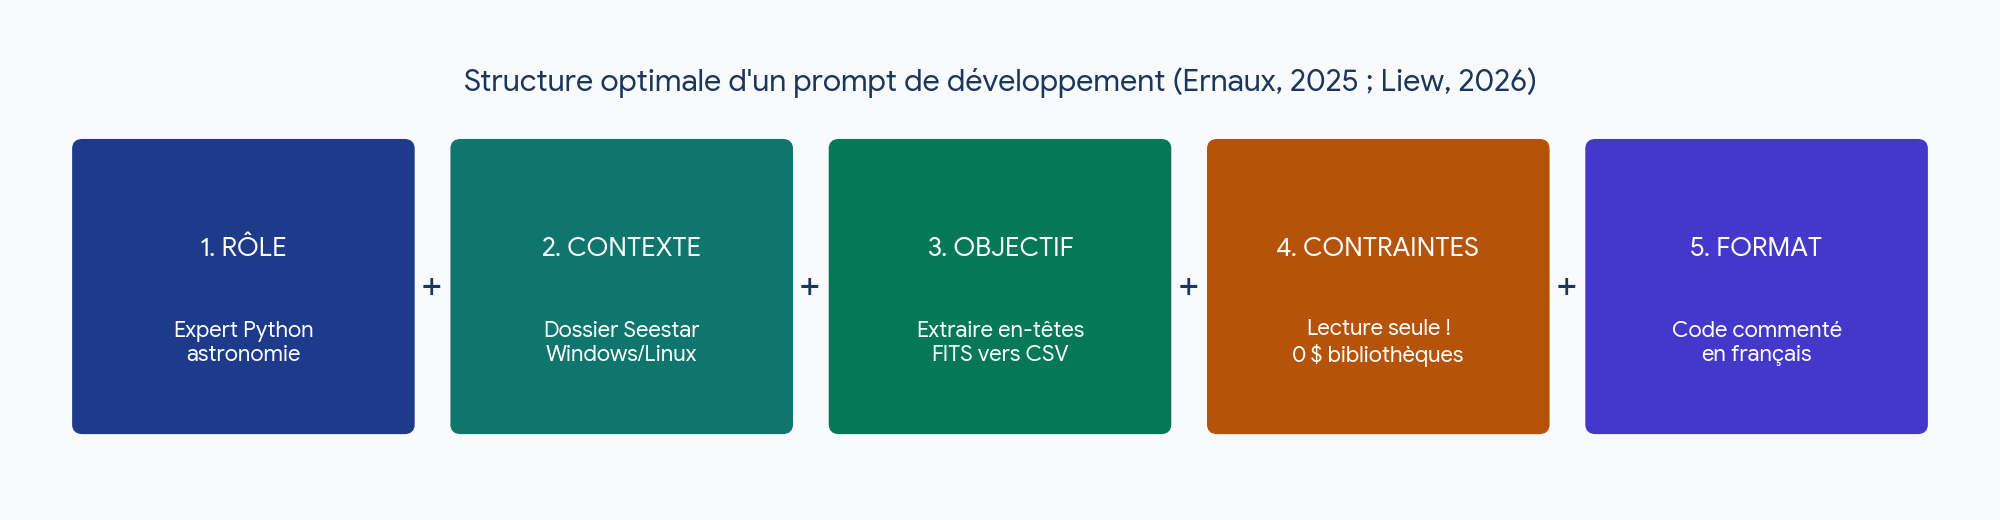
\includegraphics[width=\linewidth,height=40mm,keepaspectratio]{figures/image19.png}\par{\scriptsize Figure 20.1 — Les cinq composantes d'un prompt structuré et efficace.\par}\end{minipage}\par

\par\medskip\repere{Texte oral}

Pour passer d'une demande vague qui génère du code bancal à une instruction précise qui produit un outil fiable, les spécialistes proposent une structure claire en cinq éléments : Rôle + Contexte + Objectif + Contraintes + Format de sortie (Ernaux, 2025 ; Liew, 2026). Premièrement, attribuez un rôle (« Agis comme un développeur Python pédagogique spécialisé en astronomie ») afin d'orienter le niveau technique et le vocabulaire de l'IA (Porter et Zingaro, 2024 ; Ernaux, 2025). Deuxièmement, donnez le contexte : quel télescope utilisez-vous, sous quel système d'exploitation (Windows, Mac, Linux) et comment sont nommés vos fichiers ? Troisièmement, énoncez un objectif précis et mesurable. Quatrièmement, fixez des contraintes strictes : par exemple, « ne jamais modifier les fichiers sources », « utiliser uniquement des bibliothèques gratuites » ou « ne pas inventer de données si la météo est indisponible » (Prud'Homme, 2026b). Cinquièmement, précisez le format de sortie attendu : voulez-vous un plan d'abord, le code complet ensuite, ou des commentaires détaillés en français ? Regardez la différence entre « Fais-moi un script pour mes photos » et le prompt structuré affiché à l'écran : le second élimine toute ambiguïté (Osmani, 2025).\par

\smallskip\textbf{Animation proposée.} En binômes, ajoutez une contrainte et un critère de réussite au besoin proposé.

\clearpage\repere{DIAPOSITIVE 26 / 45 · 0:58:30 – 1:02 · 3,5 min}

{\Large\bfseries Cinq façons de préciser une demande\par}

\smallskip\hrule\smallskip

{\small\textbf{Repère visuel.} Boîte à outils des 5 techniques avancées d'ingénierie de requête.\par}

\par\medskip\repere{Texte oral}

Voici cinq techniques d'ingénierie de prompt extrêmement efficaces pour les non-développeurs. La première est le Few-Shot Prompting (l'apprentissage par l'exemple) : au lieu de décrire théoriquement à quoi ressemblent vos fichiers Seestar, copiez-collez trois vrais noms de fichiers dans votre message. L'IA comprendra immédiatement la structure exacte des dates et des numéros de catalogue (Osmani, 2025 ; Prud'Homme, 2025). La deuxième est la chaîne de pensée (Chain-of-Thought) : avant de laisser l'IA écrire cent lignes de code, demandez-lui de « réfléchir étape par étape et de vous présenter son plan d'architecture ». Vous pourrez valider la logique avant même la création du programme (Osmani, 2025 ; Liew, 2026). La troisième technique, décrite par Porter et Zingaro (2024), est l'interaction inversée : si vous ne savez pas quelles informations techniques fournir, écrivez simplement : « Je veux créer un logiciel qui calcule les meilleurs créneaux d'observation selon l'horizon de mon jardin. Pose-moi des questions une par une jusqu'à ce que tu aies tout ce qu'il faut pour le programmer. » La quatrième consiste à exiger une auto-critique de sécurité et de complétude : « Vérifie que tu n'as effacé aucune fonction existante » (Liew, 2026 ; Prud'Homme, 2026a). Enfin, la cinquième est le méta-prompting : demandez à ChatGPT de réécrire et d'optimiser votre propre requête brouillon avant de l'exécuter (Kim et Yegge, 2025 ; Liew, 2026).\par

\smallskip\textbf{Animation proposée.} Faites relire les consignes par un autre binôme. Relevez la question qui permet de lever une ambiguïté.

\clearpage\repere{DIAPOSITIVE 27 / 45 · 1:02 – 1:04:30 · 2,5 min}

{\Large\bfseries Remplacer les demandes vagues\par}

\smallskip\hrule\smallskip

{\small\textbf{Repère visuel.} Les quatre anti-patrons fréquents en Vibe Coding et comment les éviter.\par}

\par\medskip\repere{Texte oral}

À l'inverse, voici les erreurs courantes — appelées « anti-patrons » — qui provoquent les pires frustrations en Vibe Coding (Osmani, 2025 ; Ernaux, 2025). D'abord, le prompt surchargé : vouloir tout créer d'un seul bloc (la lecture FITS, la météo, la carte du ciel et le PDF) dès le premier message. L'IA va s'embrouiller et oublier la moitié des consignes. Il faut toujours procéder par petits incréments testables (Liew, 2026). Ensuite, les références floues comme « Ça ne marche pas, corrige-le » : précisez toujours quel fichier, quel bouton ou quel message d'erreur est en cause (Osmani, 2025). Troisièmement, les critères vagues : dire « Fais une belle affiche » laisse l'IA choisir des couleurs illisibles ; dites plutôt « Fond noir, texte blanc, grille de 11 colonnes par 10 rangées » (Prud'Homme, 2025). Enfin, lorsqu'une discussion devient trop longue et que l'IA s'entête dans une erreur, n'ayez pas peur de fermer la conversation et d'en ouvrir une neuve avec un contexte propre (Osmani, 2025).\par

\clearpage\repere{DIAPOSITIVE 28 / 45 · 1:04:30 – 1:09 · 4,5 min}

{\Large\bfseries Chat, Work et Codex en pratique\par}

\smallskip\hrule\smallskip

{\small\textbf{Repère visuel.} Tableau comparatif détaillé des trois modes ChatGPT (Chat, Work et Codex) selon le rôle, l'accès aux fichiers et l'usage en astronomie.\par}

\begin{minipage}[t]{.86\linewidth}\centering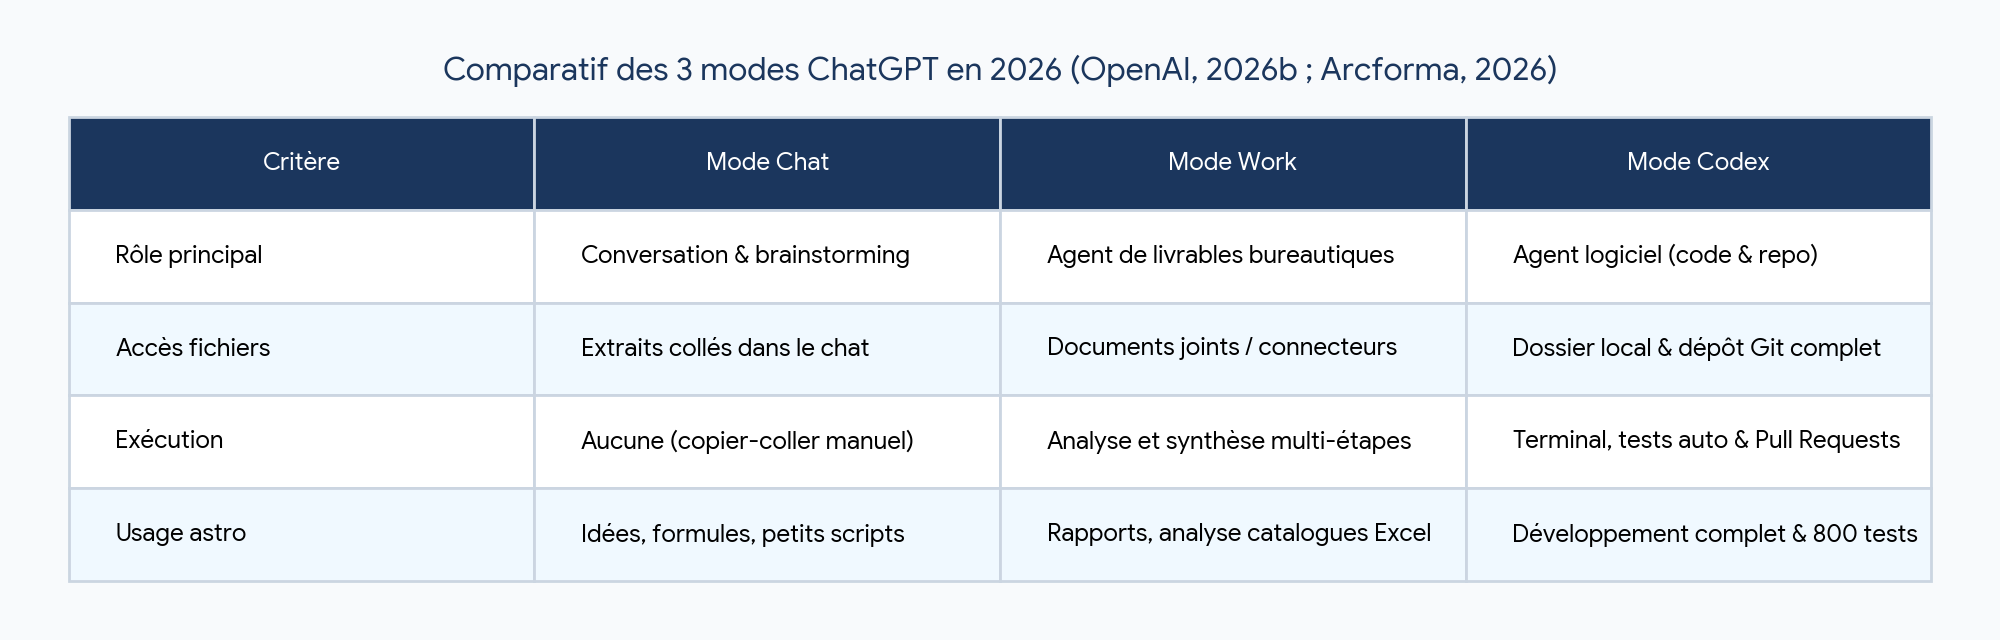
\includegraphics[width=\linewidth,height=40mm,keepaspectratio]{figures/image20.png}\par{\scriptsize Figure 23.1 — Comparatif des modes Chat, Work et Codex dans ChatGPT (OpenAI, 2026b).\par}\end{minipage}\par

\par\medskip\repere{Texte oral}

Une question que l'on me pose très souvent lorsque je présente mes projets est : « Quel outil ou quel mode utilises-tu concrètement dans ChatGPT ? » En 2026, l'écosystème OpenAI s'articule autour de trois modes distincts qui correspondent à trois niveaux de délégation différents : Chat, Work et Codex (OpenAI, 2026b ; Arcforma, 2026). Le premier est le mode Chat classique. C'est l'espace de discussion rapide. Vous posez une question, vous réfléchissez à voix haute avec l'IA, vous lui demandez d'expliquer une formule astronomique ou de générer un petit script Python de cinquante lignes que vous copiez-collez vous-même dans votre éditeur. C'est ainsi que j'ai démarré GNUAfficheMessier (Prud'Homme, 2025). L'unité de résultat du mode Chat, c'est une réponse textuelle dans le fil de conversation. Le deuxième est le mode Work. Ici, l'IA agit comme un agent autonome orienté vers la production de livrables complets en plusieurs étapes : rédiger un rapport structuré, analyser un gros tableur Excel de catalogues astronomiques, synthétiser des documents ou préparer une présentation (OpenAI, 2026b ; Politecnico di Torino, 2026). Le mode Work peut manipuler les fichiers que vous lui confiez ou auxquels vous lui donnez accès, mais il reste pensé pour la bureautique, la recherche et la gestion de projets plutôt que pour l'ingénierie logicielle pure. Le troisième, qui est une véritable révolution pour le Vibe Coding, est le mode Codex. Codex est l'agent spécialisé dans le code et les systèmes techniques, accessible dans l'application de bureau ChatGPT, sur le Web, en ligne de commande (CLI) ou dans votre éditeur de code (OpenAI, 2026b). Contrairement au mode Chat où vous devez copier-coller chaque fichier manuellement, Codex peut ouvrir directement le dossier local de votre projet sur votre ordinateur (ou cloner votre dépôt GitHub dans un bac à sable sécurisé), lire l'ensemble de vos fichiers, modifier plusieurs scripts simultanément, exécuter vos commandes dans le terminal, lancer vos centaines de tests automatisés pour vérifier qu'il n'a rien cassé, et vous présenter le résumé exact des modifications (les diffs) prêt à être publié (OpenAI, 2026b ; Arcforma, 2026). Pour résumer simplement : si vous voulez une explication ou une idée, ouvrez Chat ; si vous voulez un document ou une analyse, ouvrez Work ; si vous voulez modifier et tester un vrai projet logiciel dans vos dossiers, ouvrez Codex ! C'est grâce à cette combinaison de Chat et de Codex que j'ai pu faire évoluer GNU Astrolist jusqu'à 800 tests réussis (Prud'Homme, 2026b).\par

\smallskip\textbf{Animation proposée.} Répartissez trois tâches entre les modes : expliquer une erreur, produire une fiche, corriger un projet. Discutez les choix.

\clearpage\repere{DIAPOSITIVE 29 / 45 · 1:09 – 1:13 · 4 min}

{\Large\bfseries Comprendre le coût d'une requête\par}

\smallskip\hrule\smallskip

{\small\textbf{Repère visuel.} Graphique comparatif du coût par million de tokens (Cache vs Entrée vs Sortie) et fonctionnement des quotas partagés Work/Codex.\par}

\begin{minipage}[t]{.86\linewidth}\centering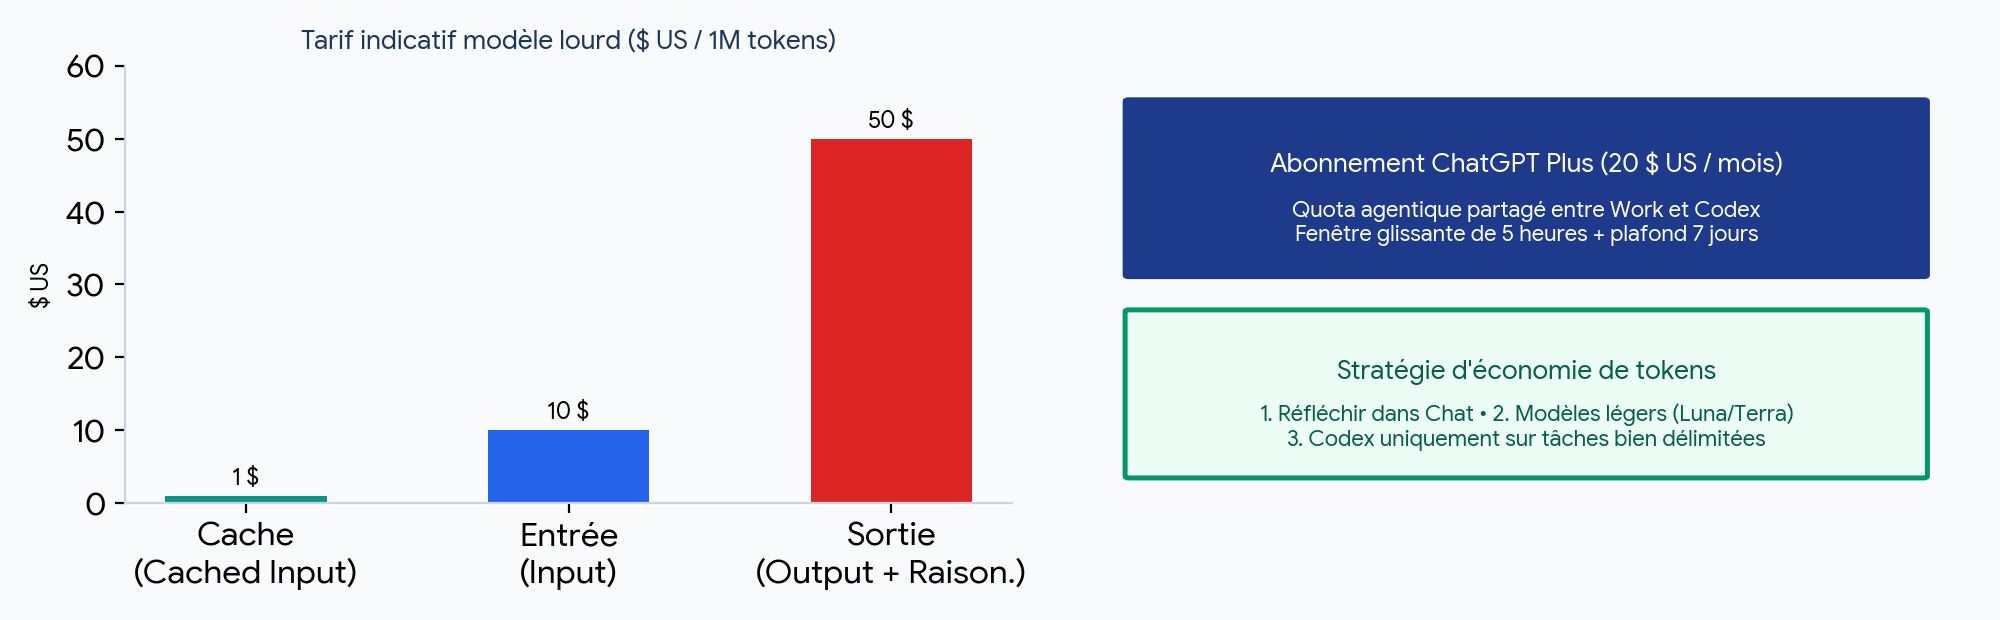
\includegraphics[width=\linewidth,height=40mm,keepaspectratio]{figures/image21.png}\par{\scriptsize Figure 24.1 — Tarification par type de tokens et gestion des quotas ChatGPT Plus (OpenAI, 2026a ; VDF.AI, 2026).\par}\end{minipage}\par

\par\medskip\repere{Texte oral}

Parlons maintenant d'un aspect très concret que tout astronome amateur soucieux de son budget doit comprendre : comment fonctionnent les tokens et combien coûte l'utilisation de ces modes ? Les modèles d'IA ne lisent pas les mots comme nous ; ils découpent le texte en petits fragments appelés tokens — environ trois quarts d'un mot en anglais, et un peu plus en français à cause des accents (Osmani, 2025). Tout ce que vous envoyez à l'IA et tout ce qu'elle vous répond est mesuré en tokens, à l'intérieur d'une mémoire temporaire appelée la fenêtre de contexte (context window). Pourquoi le mode Codex ou le mode Work consomme-t-il beaucoup plus de tokens que le mode Chat ? Parce que lorsque vous demandez à Codex de corriger un bug dans votre projet, il ne lit pas seulement votre phrase de deux lignes : il lit l'ensemble de vos fichiers Python, vos fichiers de documentation, vos tests, et il effectue souvent plusieurs étapes de raisonnement interne avant de vous répondre (Faros AI, 2026 ; Politecnico di Torino, 2026). OpenAI mesure trois types de consommation : les tokens d'entrée (ce que l'IA lit pour la première fois), les tokens mis en cache (les fichiers du projet qu'elle a déjà lus récemment, facturés jusqu'à dix fois moins cher), et les tokens de sortie, qui sont les plus coûteux et incluent la réflexion cachée du modèle (OpenAI, 2026a). En pratique, vous avez deux façons de payer. Avec un abonnement personnel comme ChatGPT Plus à 20 \$ US par mois (ou gratuit avec des limites restreintes), l'accès à Chat, Work et Codex est inclus, mais Work et Codex partagent un quota d'utilisation agentique calculé sur une fenêtre glissante de 5 heures et une fenêtre de 7 jours (VDF.AI, 2026 ; Politecnico di Torino, 2026). Si vous lancez des tâches gigantesques avec un modèle de raisonnement très lourd comme GPT-6 Astra (facturé 10 \$ en entrée et 50 \$ en sortie par million de tokens sur l'API), vous épuiserez votre quota de 5 heures en quelques requêtes ! À l'inverse, si vous utilisez des modèles rapides et économiques comme Luna ou Terra (0,10 \$ à 1 \$ par million de tokens) pour les tâches simples et gardez Sol ou Astra uniquement pour les problèmes complexes, vous économisez considérablement vos crédits (Politecnico di Torino, 2026). Mon conseil d'astronome économe : réfléchissez d'abord dans Chat, préparez vos plans, et n'activez Codex que sur des tâches bien délimitées !\par

\smallskip\textbf{Animation proposée.} Avec des tarifs fictifs de 2 et 8 dollars par million, faites chiffrer 5 000 tokens d'entrée et 1 000 de sortie. Résultat : 0,018 dollar hors taxes et cache.

\clearpage\repere{DIAPOSITIVE 31 / 45 · 1:13 – 1:17 · 4 min}

{\Large\bfseries Se repérer dans un dépôt\par}

\smallskip\hrule\smallskip

{\small\textbf{Repère visuel.} Arborescence standardisée d'un dépôt libre astronomique.\par}

\par\medskip\repere{Texte oral}

Lorsqu'on débute en Vibe Coding, on a tendance à mettre tout le code dans un seul fichier fourre-tout sur son bureau. Mais dès que le projet grandit ou que l'on souhaite le publier en logiciel libre, une organisation standardisée devient indispensable — à la fois pour les autres astronomes qui visiteront votre projet et pour l'intelligence artificielle elle-même, qui naviguera beaucoup mieux dans des modules clairs (Fogel, 2022 ; Prud'Homme, 2026a). Regardez cette arborescence type recommandée par Karl Fogel (2022) et appliquée dans mes dépôts GitHub. À la racine du dossier principal, on trouve d'abord les fichiers d'accueil et de gouvernance en lettres majuscules : README.md, LICENSE, CHANGELOG.md, CONTRIBUTING.md et ROADMAP.md. Juste en dessous, le fichier requirements.txt (ou pyproject.toml) liste les bibliothèques Python nécessaires, comme Astropy ou ReportLab, afin que n'importe quel membre du club puisse tout installer d'une seule commande (Liew, 2026). Ensuite, nous séparons proprement le code dans un dossier src/ (pour sources), les vérifications automatiques dans un dossier tests/, et les schémas ou guides dans docs/. Enfin, remarquez le fichier caché .gitignore : il est crucial en astronomie ! Il indique à Git d'ignorer vos fichiers temporaires, vos caches météo et surtout vos gigaoctets de photos brutes FITS ou JPEG, afin de ne publier sur Internet que le code léger du logiciel et non pas votre disque dur entier !\par

\smallskip\textbf{Animation proposée.} Faites retrouver le dossier où placer un exemple puis celui où vérifier un résultat.

\clearpage\repere{DIAPOSITIVE 32 / 45 · 1:17 – 1:23 · 6 min}

{\Large\bfseries Cinq fichiers pour travailler ensemble\par}

\smallskip\hrule\smallskip

{\small\textbf{Repère visuel.} Rôle des 5 fichiers Markdown (.md) dans la gouvernance humaine et la configuration de l'agent IA.\par}

\par\medskip\repere{Texte oral}

Attardons-nous un instant sur ces fichiers qui se terminent par l'extension .md, pour Markdown. Comme le souligne Karl Fogel (2022), le Markdown est devenu le standard universel de documentation du monde open source. C'est un fichier texte tout simple dans lequel on utilise des symboles légers — comme un dièse \# pour un titre ou deux astérisques ** pour mettre en gras — afin de structurer un document sans avoir besoin d'un traitement de texte lourd. Dès que vous déposez un fichier .md sur GitHub, la plateforme le met automatiquement en page de manière élégante. Quels sont les fichiers .md essentiels que vous devriez demander à ChatGPT de générer pour chacun de vos projets ? Le premier, obligatoire, est le README.md (« Lisez-moi »). C'est la vitrine de votre projet. Lorsqu'un astronome arrive sur votre page GitHub, c'est le premier texte qu'il lit. Un bon README.md répond à quatre questions : à quoi sert ce logiciel, comment l'installer, comment lancer une première commande d'exemple, et sous quelle licence libre il est distribué (Liew, 2026 ; Fogel, 2022). Le deuxième est le CHANGELOG.md (journal des modifications). À chaque nouvelle version, on y note ce qui a été ajouté, modifié ou corrigé. Cela permet aux utilisateurs de suivre l'évolution de l'outil (Prud'Homme, 2025). Le troisième est le ROADMAP.md (feuille de route). C'est là que vous notez vos idées futures — par exemple, dans GNU Astro Galery, l'ajout prévu de l'échelle de Bortle ou du seeing (Prud'Homme, 2026a). Cela évite de tout vouloir faire en même temps et montre aux autres contributeurs où va le projet. Le quatrième, lorsque le projet grandit, est le CONTRIBUTING.md (et parfois CODE\_OF\_CONDUCT.md), qui explique comment un autre passionné peut vous aider, signaler une erreur de catalogue ou proposer une correction (Eghbal, 2020). Enfin, le Vibe Coding a fait naître un cinquième fichier Markdown extrêmement précieux : le fichier de consignes pour l'IA, souvent nommé AGENTS.md (ou INSTRUCTIONS.md) placé à la racine du projet (Osmani, 2025). Plutôt que de répéter à chaque nouvelle conversation avec ChatGPT ou Codex : « Attention, ne touche jamais aux fichiers FITS originaux, écris les messages d'erreur en français et n'invente jamais une magnitude manquante », vous inscrivez ces règles d'or dans ce fichier Markdown. À chaque session, l'agent IA le lit automatiquement avant de toucher à une seule ligne de code ! Et la meilleure nouvelle dans tout ça ? Vous n'avez même pas à rédiger ces fichiers .md à la main : vous demandez à l'IA de les générer et de les mettre à jour pour vous (Liew, 2026).\par

\smallskip\textbf{Animation proposée.} Attribuez les cinq fichiers à cinq personnes. Chacune propose une première phrase utile au club.

\clearpage\repere{DIAPOSITIVE 34 / 45 · 1:23 – 1:26 · 3 min}

{\Large\bfseries Git conserve l'historique du projet\par}

\smallskip\hrule\smallskip

{\small\textbf{Repère visuel.} Distinction entre Git (contrôle de version local hors ligne) et GitHub (hébergement et partage communautaire en ligne).\par}

\par\medskip\repere{Texte oral}

Si vous ne devez retenir qu'une seule règle technique de cette soirée pour éviter les crises de nerfs face à l'IA, c'est celle-ci : utilisez Git et GitHub dès la première minute de votre projet (Liew, 2026 ; Prud'Homme, 2026a). On confond souvent les deux termes, mais leur distinction est très simple (Eghbal, 2020). Git est un logiciel libre installé localement sur votre propre ordinateur (Windows, Mac ou Linux). Créé en 2005 par Linus Torvalds pour gérer le développement du noyau Linux, Git est une véritable machine à remonter le temps pour vos dossiers de code : il enregistre chaque étape de votre travail sur votre disque dur, même lorsque vous êtes en plein champ sous les étoiles sans connexion Internet (Martin et Newkirk, 2025). GitHub, quant à lui, est un site Web (une plateforme d'hébergement) où vous envoyez une copie de votre dépôt Git pour le sauvegarder en sécurité, le partager publiquement avec d'autres astronomes, recevoir des signalements de bugs (Issues) ou accepter des améliorations (Pull Requests) (Fogel, 2022). Pourquoi est-ce vital en Vibe Coding ? Parce que, comme nous l'avons vu, l'IA peut parfois effacer 30 \% de votre code en une seule réponse (Prud'Homme, 2026a). Avec Git, vous revenez à la version fonctionnelle d'il y a cinq minutes en une fraction de seconde !\par

\clearpage\repere{DIAPOSITIVE 35 / 45 · 1:26 – 1:30 · 4 min}

{\Large\bfseries Enregistrer un changement avec Git\par}

\smallskip\hrule\smallskip

{\small\textbf{Repère visuel.} Chaîne chronologique des commits Git permettant de restaurer une version saine après une erreur IA.\par}

\begin{minipage}[t]{.86\linewidth}\centering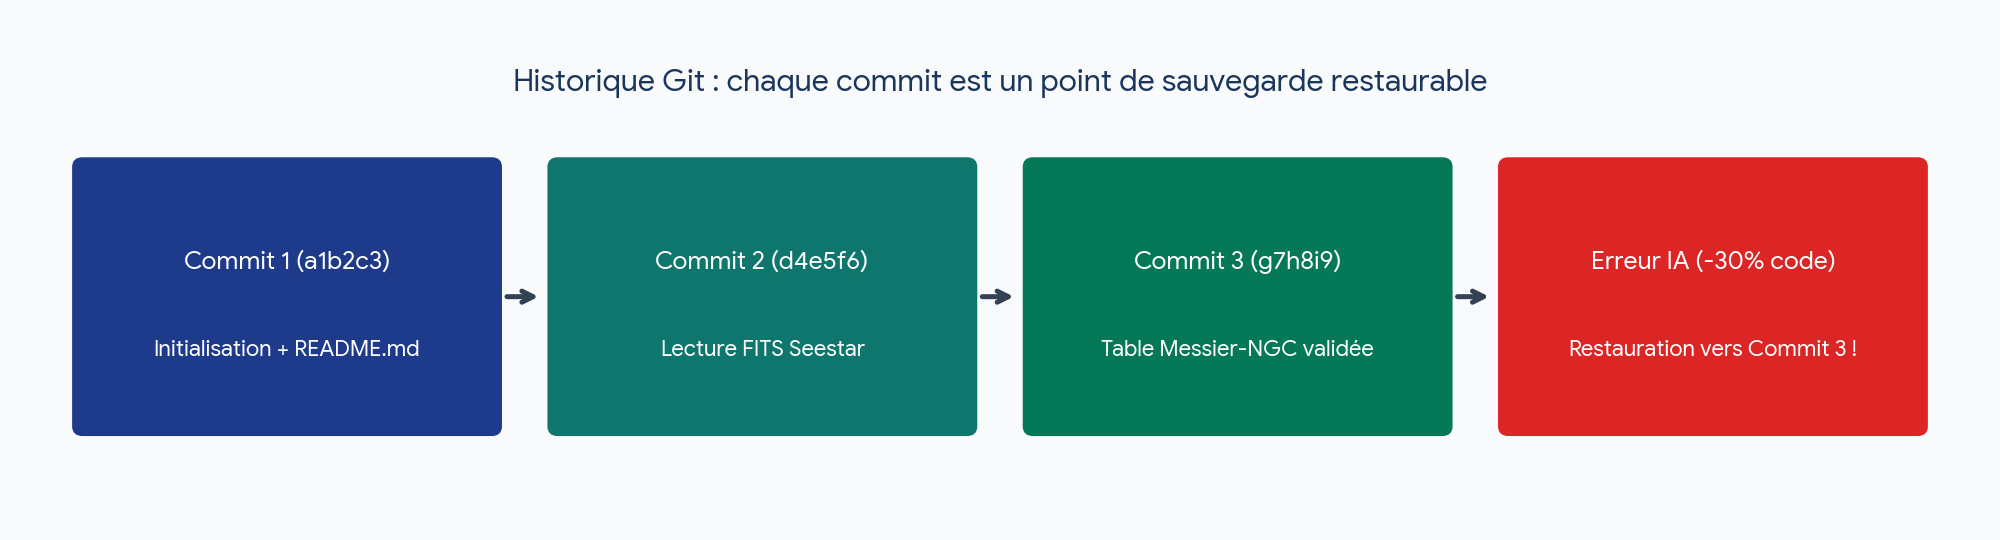
\includegraphics[width=\linewidth,height=40mm,keepaspectratio]{figures/image22.png}\par{\scriptsize Figure 28.1 — Historique des commits et restauration rapide en cas d'erreur de l'IA.\par}\end{minipage}\par

\par\medskip\repere{Texte oral}

Le concept central de Git, c'est le commit (que l'on traduit parfois par « validation » ou « instantané »). Comme l'explique Karl Fogel (2022), faire un commit, c'est prendre une photographie complète et datée de l'état de tous vos fichiers à un instant précis, en y attachant une courte étiquette descriptive — le message de commit — qui explique pourquoi vous avez fait cette modification. Contrairement à un simple « Enregistrer » dans Word qui écrase la version précédente, Git empile ces photographies les unes à la suite des autres dans un journal historique inaltérable. Beaucoup de débutants ont peur du terminal (l'écran noir où l'on tape des commandes), mais pour gérer 95 \% de vos projets en Vibe Coding, vous n'avez besoin que de quatre commandes très simples, affichées à l'écran (Liew, 2026). Au tout début du projet, vous tapez git init pour activer le suivi dans votre dossier. Ensuite, dès que vous avez testé une fonctionnalité générée par l'IA et qu'elle fonctionne, vous tapez git add . pour sélectionner les fichiers modifiés, puis git commit -m "Votre message clair" pour sceller ce point de sauvegarde (Liew, 2026). Évitez les messages vagues comme "update" ou "test" ; écrivez plutôt "Ajout du filtrage des dossiers -sub" afin de vous y retrouver trois mois plus tard ! Enfin, la commande git push expédie vos commits locaux vers votre page GitHub pour les mettre à l'abri en ligne. Et si vous n'aimez pas le terminal, sachez que des logiciels gratuits comme Visual Studio Code ou GitHub Desktop permettent de faire exactement la même chose en cliquant sur un bouton !\par

\smallskip\textbf{Animation proposée.} Montrez git status avant et après avoir choisi un fichier. Repérez ensemble le nom du fichier prêt pour le commit.

\clearpage\repere{DIAPOSITIVE 36 / 45 · 1:30 – 1:33:30 · 3,5 min}

{\Large\bfseries Essayer une idée sur une branche\par}

\smallskip\hrule\smallskip

{\small\textbf{Repère visuel.} Diagramme de branchement Git : branche principale (main) vs branche d'essai isolée.\par}

\begin{minipage}[t]{.86\linewidth}\centering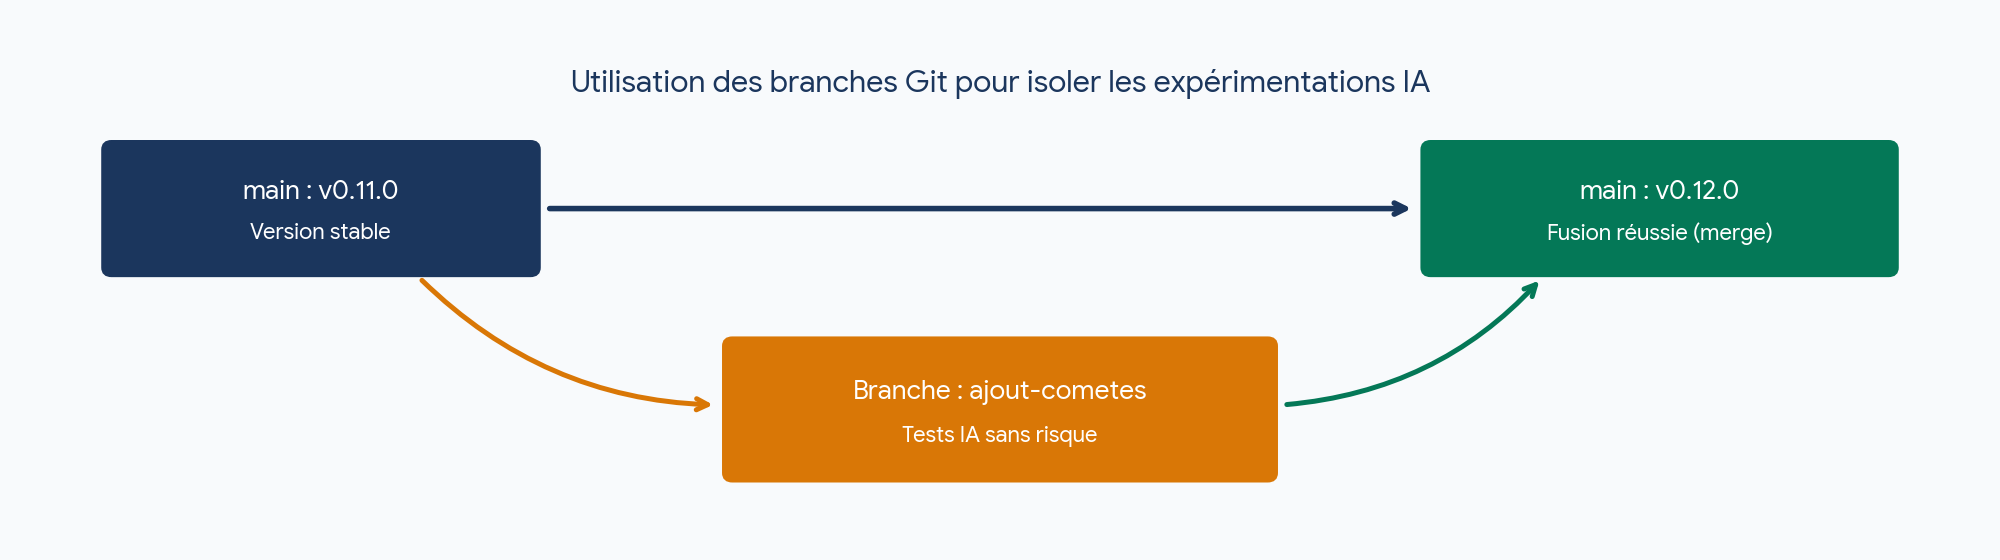
\includegraphics[width=\linewidth,height=40mm,keepaspectratio]{figures/image23.png}\par{\scriptsize Figure 29.1 — Isolation des expérimentations IA grâce aux branches Git (Fogel, 2022).\par}\end{minipage}\par

\par\medskip\repere{Texte oral}

Pourquoi insistons-nous autant sur le fait de commiter très fréquemment lorsqu'on développe avec une intelligence artificielle ? Martin et Newkirk (2025) rappellent qu'avec Git, faire un commit local est instantané et gratuit : vous pouvez en faire un toutes les dix minutes, dès qu'un petit test réussit. En Vibe Coding, c'est votre bouée de sauvetage. Avant de demander à ChatGPT ou à Codex de réorganiser votre programme ou d'ajouter un nouveau catalogue astronomique, faites toujours un commit de votre version qui fonctionne (Liew, 2026). Si l'IA casse tout, vous tapez git checkout . ou git reset -{}-hard et l'incident est effacé. De plus, lorsque vous voulez expérimenter une fonctionnalité complexe sans risquer de déstabiliser votre logiciel principal, Git offre un outil merveilleux appelé la branche (branch). Karl Fogel (2022) compare la branche principale (main) au château central que tout le monde utilise, et une branche secondaire (git checkout -b ajout-cometes) à un terrain d'essai isolé où vous pouvez construire un nouveau pont-levis. Si le pont-levis tient debout après vos tests, vous le fusionnez (merge) dans le château principal ; s'il s'effondre, vous supprimez simplement la branche d'essai sans aucun dégât !\par

\clearpage\repere{DIAPOSITIVE 37 / 45 · 1:33:30 – 1:37 · 3,5 min}

{\Large\bfseries Lire un numéro de version\par}

\smallskip\hrule\smallskip

{\small\textbf{Repère visuel.} Schéma explicatif SemVer extrait des notes de conférence GNU Astrolist (Prud'Homme, 2026b, section 05).\par}

\begin{minipage}[t]{.86\linewidth}\centering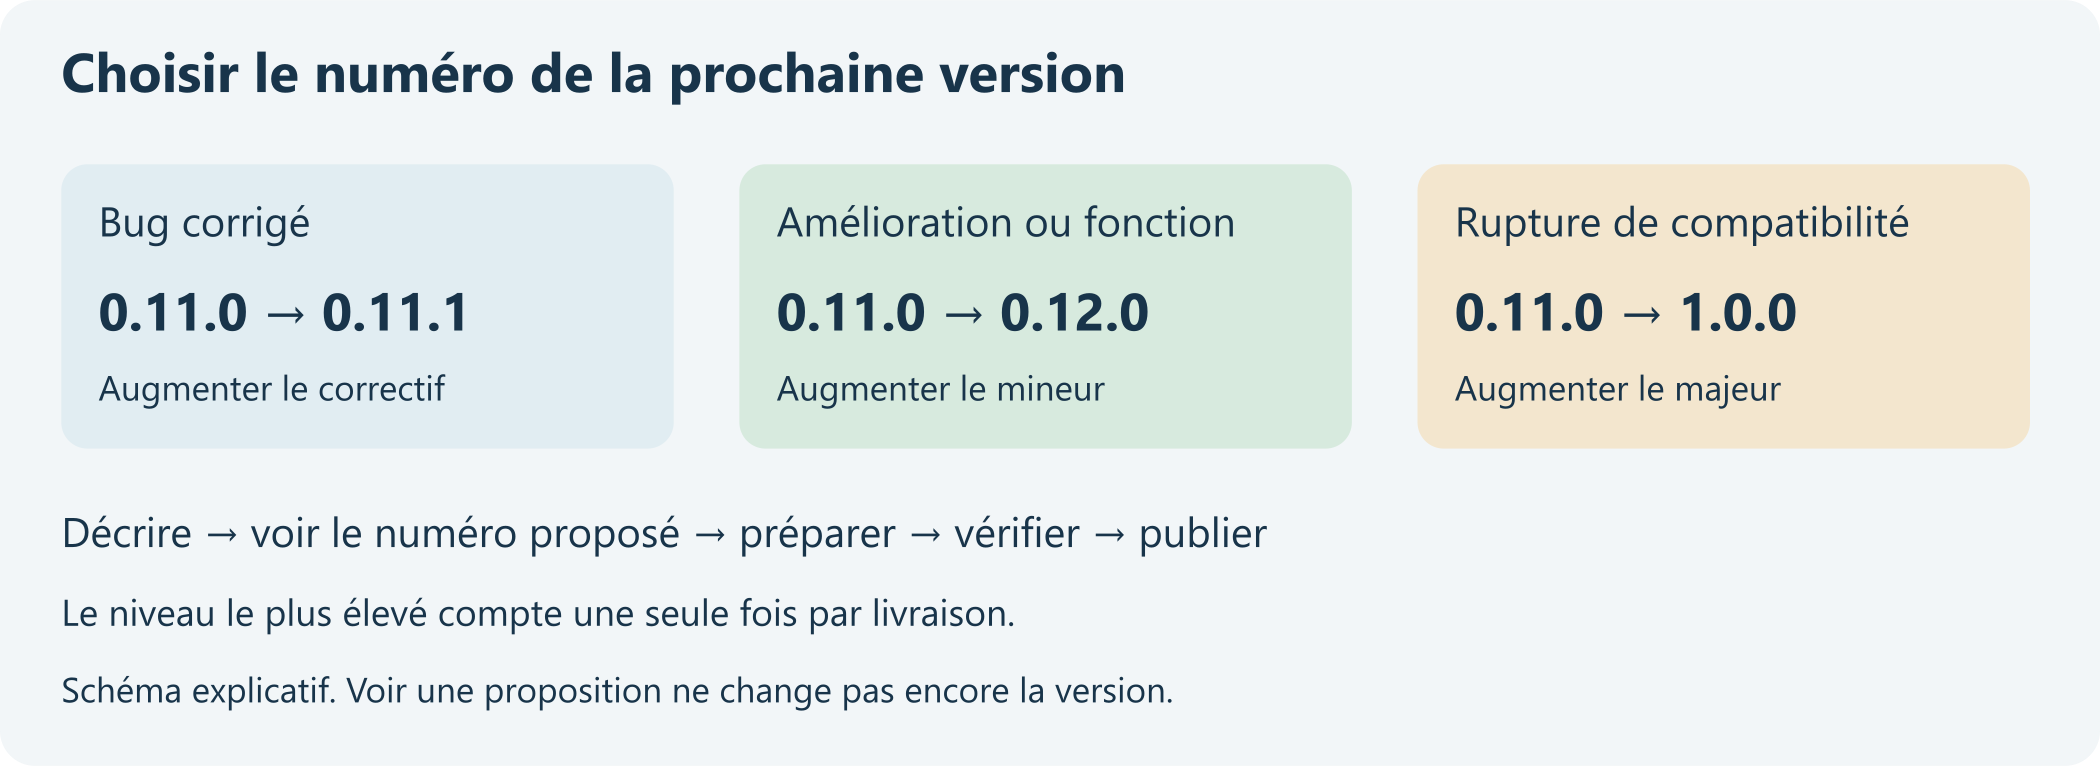
\includegraphics[width=\linewidth,height=40mm,keepaspectratio]{figures/image24.png}\par{\scriptsize Figure 30.1 — Règles de numérotation sémantique SemVer appliquées à GNU Astrolist (Prud'Homme, 2026b).\par}\end{minipage}\par

\par\medskip\repere{Texte oral}

Enfin, comment numéroter proprement les étapes de vie de notre logiciel pour que les membres du club sachent s'ils téléchargent un brouillon expérimental ou un outil stable ? Dans le monde du logiciel libre, on utilise une convention très claire appelée le versionnement sémantique (SemVer), illustrée par ce schéma tiré de mon projet GNU Astrolist (Prud'Homme, 2026b). Un numéro de version comporte trois chiffres séparés par des points, par exemple 0.11.0 : MAJEUR . MINEUR . CORRECTIF. Tant que le premier chiffre est un zéro (comme 0.0.1 pour GNUAfficheMessier ou 0.8.0 pour Astro Galery), cela signale honnêtement aux autres astronomes que le logiciel est en phase de développement actif (état alpha ou bêta décrit par Fogel, 2022). Lorsque vous corrigez simplement un petit bug sans rien changer d'autre, vous augmentez le troisième chiffre : 0.11.0 devient 0.11.1 (le correctif). Lorsque vous ajoutez une nouvelle capacité compatible — par exemple la prise en charge des comètes —, vous augmentez le chiffre du milieu et remettez le dernier à zéro : 0.12.0 (la version mineure). Et le jour où votre outil est mûr, validé scientifiquement et stabilisé pour le grand public, vous publiez la célèbre version 1.0.0 (la version majeure) ! Par la suite, vous n'augmenterez le chiffre majeur (2.0.0) que si vous modifiez le fonctionnement du logiciel d'une façon qui oblige les utilisateurs à changer leurs habitudes.\par

\clearpage\repere{DIAPOSITIVE 38 / 45 · 1:37 – 1:39 · 2 min}

{\Large\bfseries Quatre projets de vibe coding en astronomie\par}

\smallskip\hrule\smallskip

{\small\textbf{Repère visuel.} Présentation synthétique des quatre dépôts GitHub développés pour le Seestar S50.\par}

\par\medskip\repere{Texte oral}

Il est temps maintenant de passer de la théorie à la réalité du terrain ! Au cours de la dernière année, pour répondre à mes propres besoins d'astrophotographe utilisant un télescope intelligent Seestar S50, j'ai développé et publié quatre projets libres sur mon compte GitHub, tous conçus grâce au Vibe Coding. Chacun de ces projets illustre une facette différente de la collaboration avec l'IA : un utilitaire graphique créé en une journée (GNUAfficheMessier), un générateur de site Web scientifique (GNU Astro Galery), la reprise et la modernisation d'un ancien logiciel avec Codex (GNU Astrolist), et enfin la valorisation locale des archives FITS brutes (GNU Astrophotography Recycle). Explorons-les ensemble en détail.\par

\smallskip\textbf{Animation proposée.} Demandez quel projet répond au besoin le plus fréquent du club.

\clearpage\repere{DIAPOSITIVE 39 / 45 · 1:39 – 1:41:30 · 2,5 min}

{\Large\bfseries Une affiche pour suivre ses objets Messier\par}

\smallskip\hrule\smallskip

{\small\textbf{Repère visuel.} Maquette illustrative de l'affiche 24 \(\times\) 36 pouces, schéma de la structure MyWorks du Seestar S50 et équivalence M31 = NGC 224 (Prud'Homme, 2025).\par}

\begin{minipage}[t]{.48\linewidth}\centering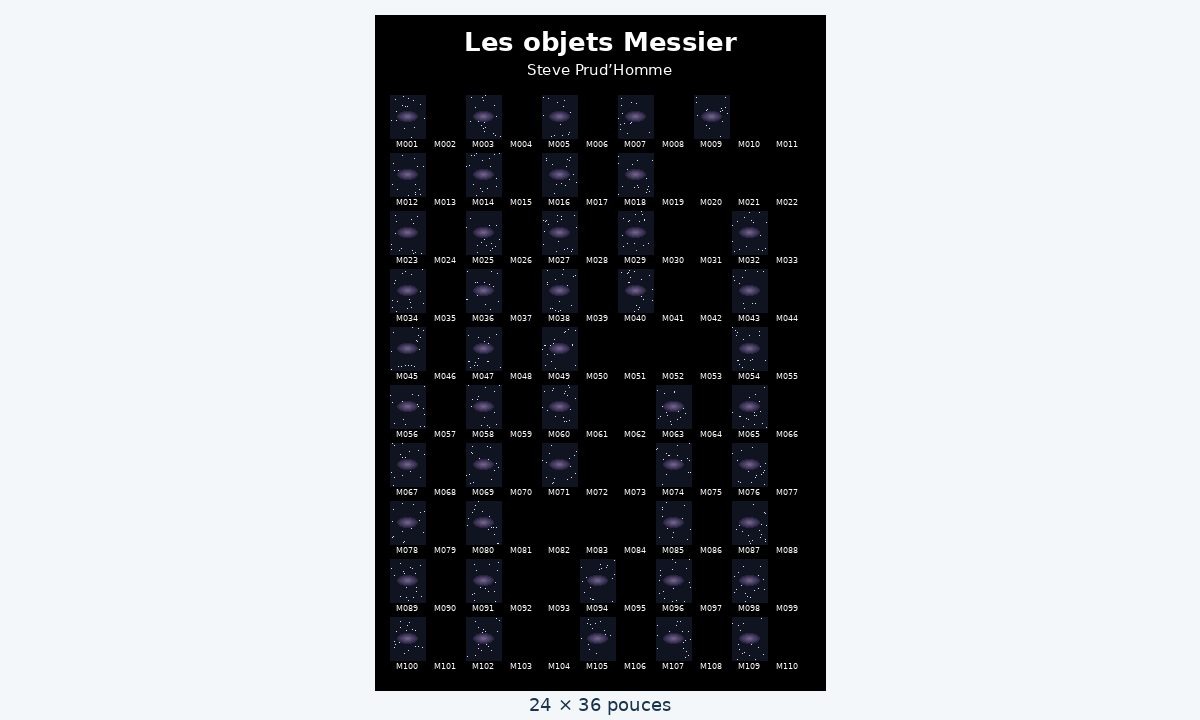
\includegraphics[width=\linewidth,height=28mm,keepaspectratio]{figures/image25.png}\par{\scriptsize Figure 32.1 — Maquette illustrative de l'affiche murale 24 \(\times\) 36 pouces « Les objets Messier » (Prud'Homme, 2025).\par}\end{minipage}\hfill

\begin{minipage}[t]{.48\linewidth}\centering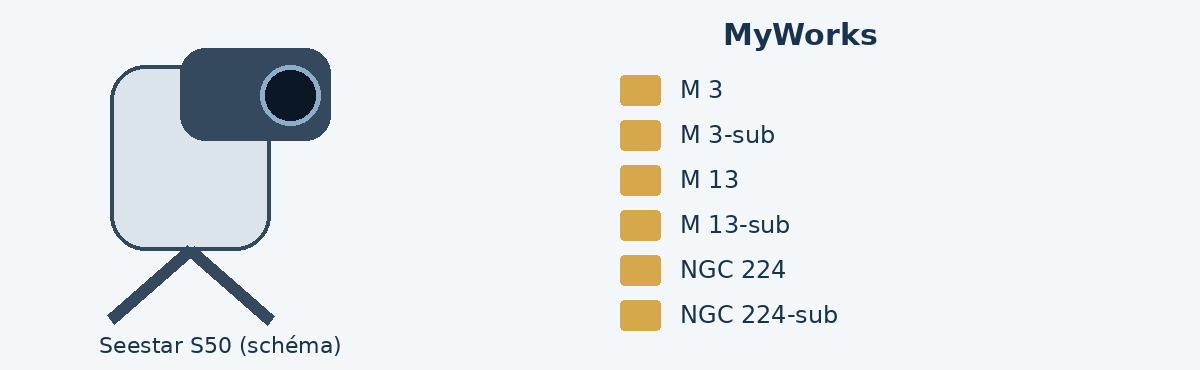
\includegraphics[width=\linewidth,height=28mm,keepaspectratio]{figures/image26.png}\par{\scriptsize Figure 32.2 — Schéma du Seestar S50 et organisation des répertoires MyWorks et -sub (Prud'Homme, 2025).\par}\end{minipage}\par

\begin{minipage}[t]{.48\linewidth}\centering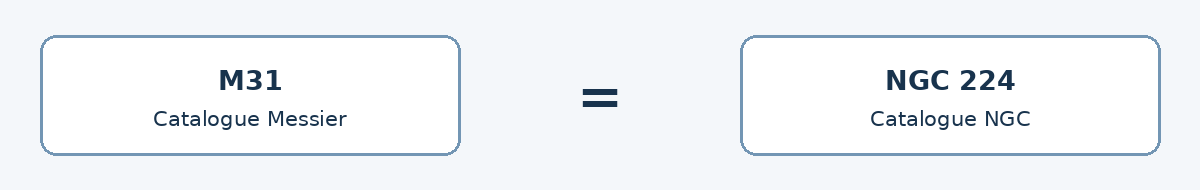
\includegraphics[width=\linewidth,height=28mm,keepaspectratio]{figures/image27.png}\par{\scriptsize Figure 32.3 — Double désignation astronomique : M31 (Messier) = NGC 224 (New General Catalogue) (Prud'Homme, 2025).\par}\end{minipage}\hfill

\par\medskip\repere{Texte oral}

Le premier projet est GNUAfficheMessier. Comme beaucoup d'entre vous qui possédez un Seestar S50, j'ai vite accumulé une montagne de fichiers dans le dossier MyWorks : lors d'un premier balayage, mon disque contenait 18 024 fichiers JPEG ! Pourquoi autant ? Parce que le télescope sauvegarde non seulement l'image empilée finale, mais aussi des vignettes et des centaines de poses individuelles dans des sous-dossiers terminés par \_sub ou -sub (Prud'Homme, 2025). Mon rêve était simple : produire une grande affiche murale de 24 par 36 pouces présentant les 110 objets du catalogue Messier dans une grille fixe, avec mes propres photos dans les cases réussies et du noir dans les cases encore à photographier. Mais un piège astronomique guettait : le Seestar enregistre parfois la galaxie d'Andromède sous le nom M 31 et parfois sous NGC 224. Il fallait donc un programme capable de filtrer les déchets, de réconcilier les catalogues Messier et NGC, et de composer le PDF automatiquement (Prud'Homme, 2025).\par

\smallskip\textbf{Animation proposée.} Suivez les deux noms de la galaxie sur la maquette. Repérez où un doublon fausserait le bilan.

\clearpage\repere{DIAPOSITIVE 40 / 45 · 1:41:30 – 1:44:30 · 3 min}

{\Large\bfseries 04 — La première conversation avec ChatGPT\par}

\smallskip\hrule\smallskip

{\small\textbf{Repère visuel.} Chaîne de traitement automatisée et statistiques du premier essai de GNUAfficheMessier (18 024 JPEG recensés, 35/110 objets = 31,8 \%).\par}

\begin{minipage}[t]{.48\linewidth}\centering
\includegraphics[width=\linewidth,height=28mm,keepaspectratio]{figures/image28.png}\par{\scriptsize Figure 33.1 — Chaîne de traitement automatisée : MyWorks \(\rightarrow\) GNUAfficheMessier \(\rightarrow\) Affiche PDF (Prud'Homme, 2025).\par}\end{minipage}\hfill

\begin{minipage}[t]{.48\linewidth}\centering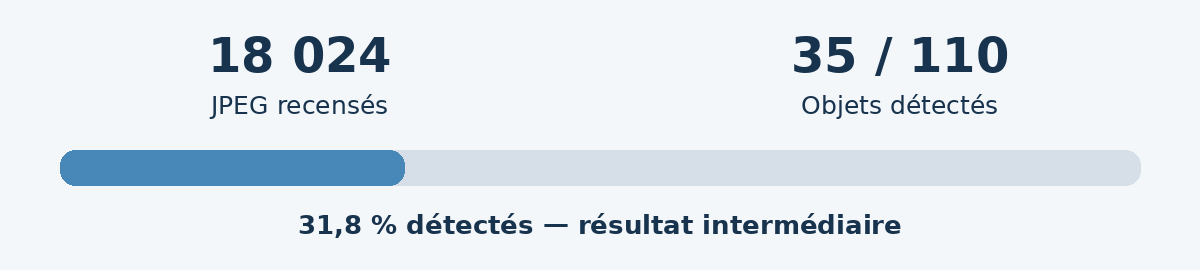
\includegraphics[width=\linewidth,height=28mm,keepaspectratio]{figures/image29.png}\par{\scriptsize Figure 33.2 — Statistiques intermédiaires du premier essai : 35 objets Messier détectés sur 110 (Prud'Homme, 2025).\par}\end{minipage}\par

\par\medskip\textbf{À projeter.} Après le bilan du premier essai, montrez le PDF réalisé. Avancez encore pour agrandir une rangée. Faites distinguer une case photographiée et une case en attente.\par\medskip
\repere{Texte oral}

Regardez cette diapositive : je tiens à vous montrer le véritable message initial que j'ai envoyé à ChatGPT le 29 décembre 2025 pour lancer ce projet. Vous voyez qu'il n'y a aucune formule magique, pas de jargon technique, et même quelques fautes de frappe (« sript », « parmis ») ! Comme le confirment Kim et Yegge (2025), les modèles modernes tolèrent parfaitement les fautes d'orthographe et extraient votre intention. À partir de ces quatre phrases, ChatGPT a immédiatement compris qu'il fallait utiliser Python avec les bibliothèques gratuites Pillow et ReportLab, et il a calculé qu'une grille de 11 colonnes par 10 rangées permettait d'afficher les 110 objets sur un poster 24 par 36 pouces (Prud'Homme, 2025). Bien sûr, tout n'a pas fonctionné du premier coup : il a fallu plusieurs allers-retours pour passer les noms des objets en français, corriger le filtrage des dossiers -sub et réparer les trois erreurs scientifiques de la table NGC que nous avons vues plus tôt. Mais en une journée, l'outil fonctionnait !\par

\smallskip\textbf{Animation proposée.} Faites expliquer ce que signifie 35 sur 110. Demandez quelle vérification manuelle ferait gagner confiance.

\clearpage\repere{DIAPOSITIVE 41 / 45 · 1:44:30 – 1:49 · 4,5 min}

{\Large\bfseries Du fichier FITS à la galerie Web\par}

\smallskip\hrule\smallskip

{\small\textbf{Repère visuel.} Captures originales du projet GNU Astro Galery : interface Web de la galerie, répertoire M 44, en-tête FITS dans FITS Liberator et carte stellaire M 102.\par}

\begin{minipage}[t]{.48\linewidth}\centering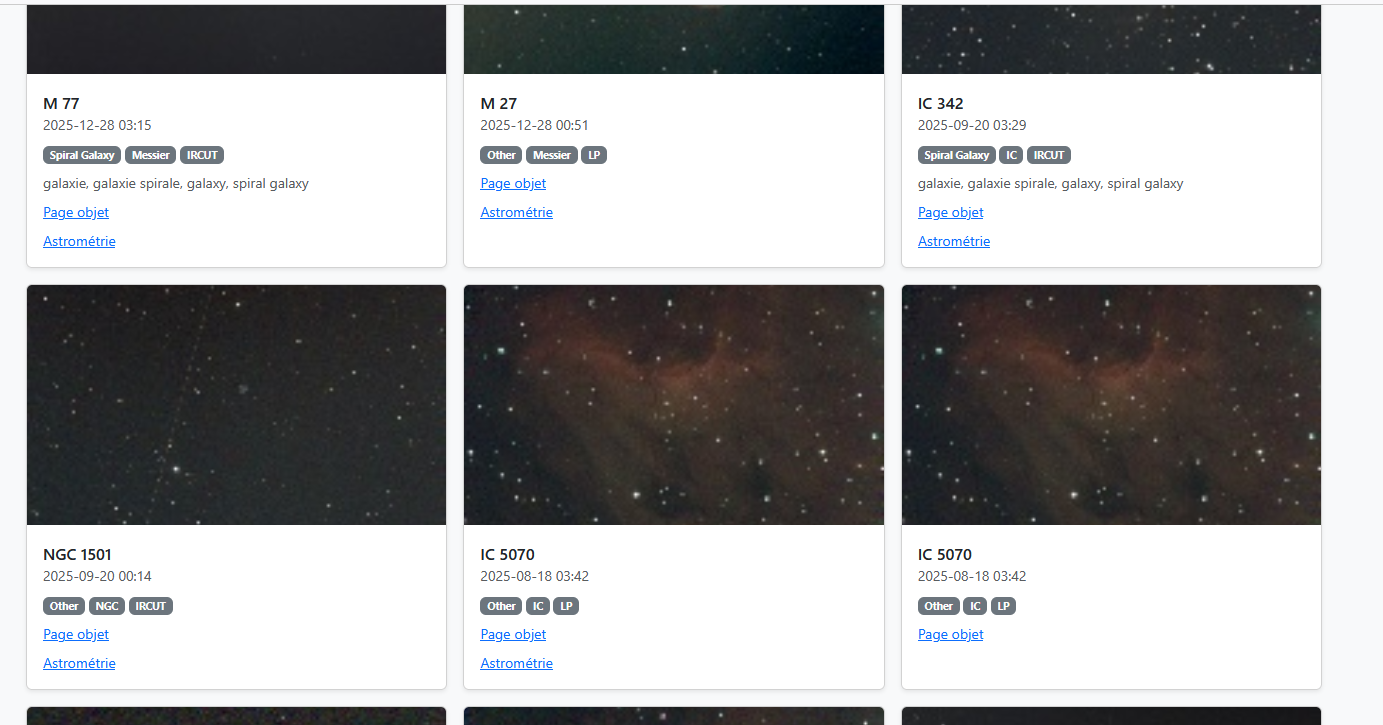
\includegraphics[width=\linewidth,height=28mm,keepaspectratio]{figures/image30.png}\par{\scriptsize Figure 34.1 — Interface Web réelle de GNU Astro Galery (M 77, M 27, IC 342, NGC 1501, IC 5070) (Prud'Homme, 2026a).\par}\end{minipage}\hfill

\begin{minipage}[t]{.48\linewidth}\centering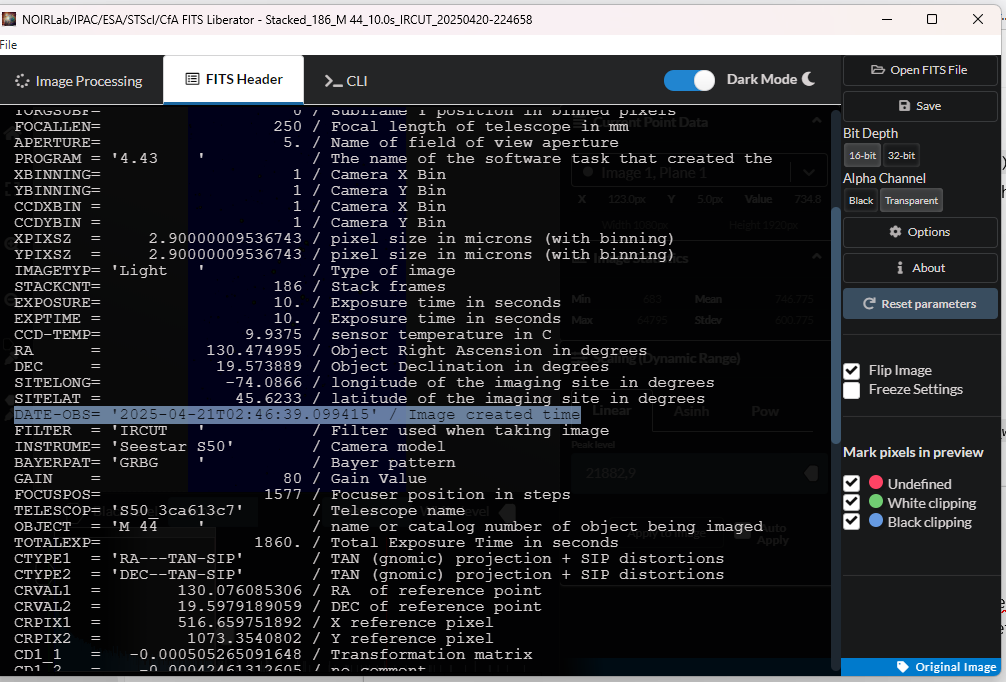
\includegraphics[width=\linewidth,height=28mm,keepaspectratio]{figures/image31.png}\par{\scriptsize Figure 34.2 — Contenu d'un répertoire d'observation Seestar S50 (M 44 : fichiers .fit, .jpg et miniature) (Prud'Homme, 2026a).\par}\end{minipage}\par

\begin{minipage}[t]{.48\linewidth}\centering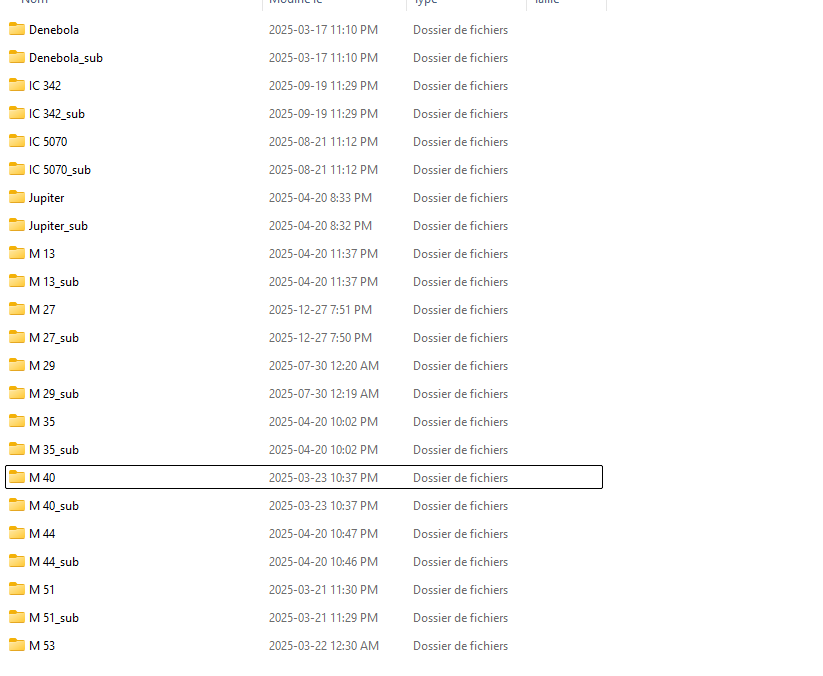
\includegraphics[width=\linewidth,height=28mm,keepaspectratio]{figures/image32.png}\par{\scriptsize Figure 34.3 — Métadonnées astronomiques extraites de l'en-tête FITS (RA, DEC, EXPTIME, DATE-OBS, IRCUT) (Prud'Homme, 2026a).\par}\end{minipage}\hfill

\begin{minipage}[t]{.48\linewidth}\centering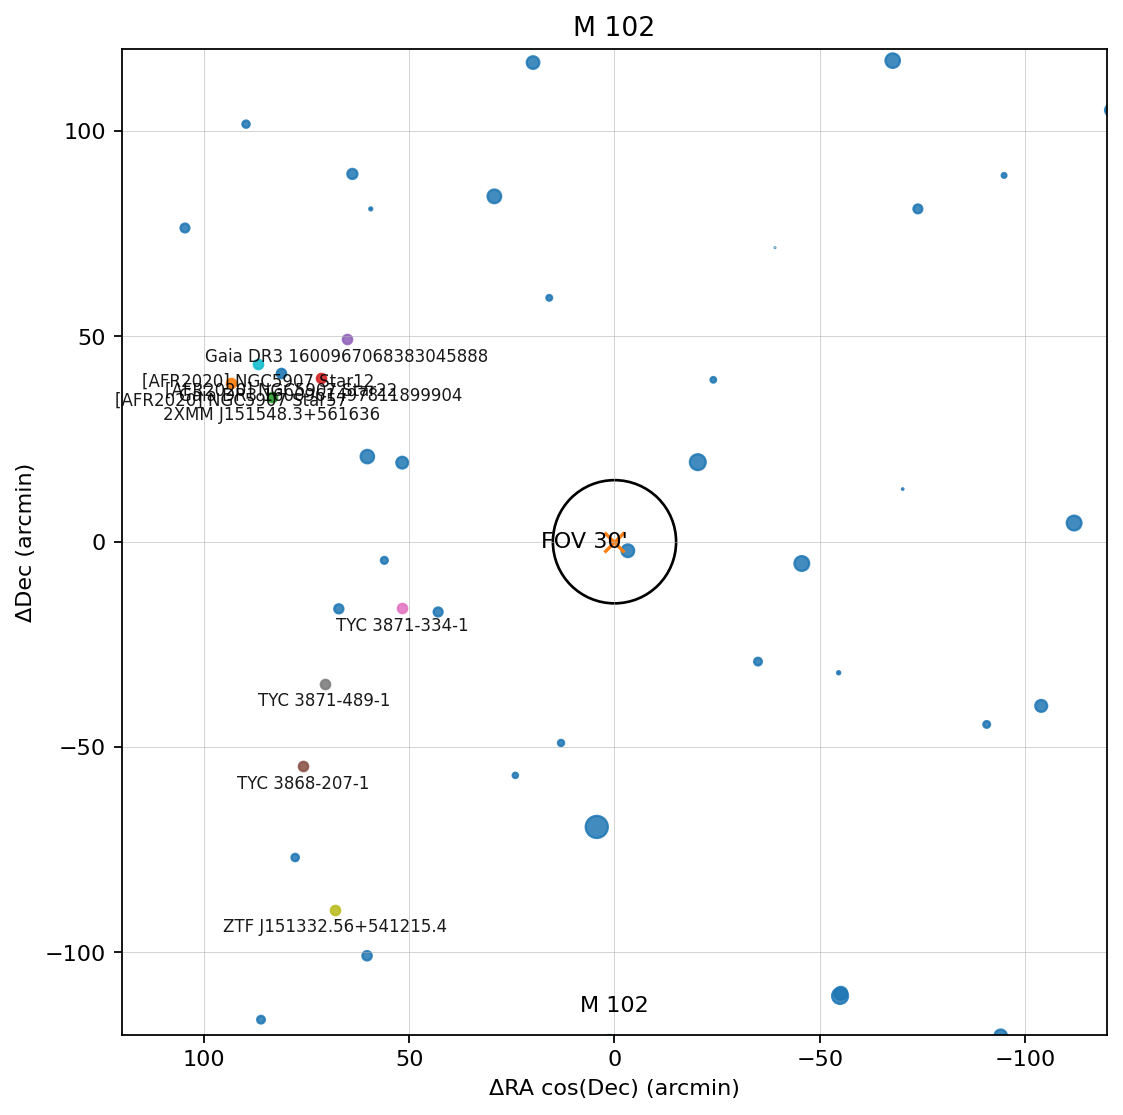
\includegraphics[width=\linewidth,height=28mm,keepaspectratio]{figures/image18.png}\par{\scriptsize Figure 34.4 — Carte stellaire centrée sur M 102 générée automatiquement par Matplotlib (Prud'Homme, 2026a).\par}\end{minipage}\par

\par\medskip\textbf{À projeter.} Affichez les quatre vues successives : répertoire de M44, en-tête FITS, carte de M102 et galerie finale. Ces objets illustrent des étapes différentes.\par\medskip
\repere{Texte oral}

Le deuxième projet est GNU Astro Galery. Lorsque l'on partage une astrophotographie sur Facebook ou Instagram, on perd toute sa richesse scientifique : le temps de pose total, le filtre utilisé, la température du capteur, les coordonnées célestes exactes et la météo qu'il faisait cette nuit-là. Pourtant, toutes ces informations sont précieusement enregistrées à l'intérieur du fichier FITS produit par le télescope ! J'ai donc demandé à ChatGPT de m'aider à créer un programme Python qui scanne mes dossiers d'observation — comme celui de l'amas de la Crèche M 44 que vous voyez à l'écran —, lit les en-têtes FITS grâce à Astropy, interroge les catalogues SIMBAD et Open-Meteo pour retrouver la météo historique de la soirée, trace une carte du ciel autour de l'objet avec Matplotlib et génère un site Web statique complet prêt à être mis en ligne (Prud'Homme, 2026a). Ce projet m'a appris deux leçons fondamentales du Vibe Coding. D'abord, la valeur de la mise en cache : au début, le programme retéléchargeait toutes les données sur Internet à chaque exécution ; en expliquant simplement le problème à ChatGPT, il a créé une mémoire locale qui accélère tout. Ensuite, l'importance de la modularité et de Git : c'est sur ce projet, en version 0.8.0, que ChatGPT a effacé 30 \% de mon fichier de 86 Ko lors d'une refonte, me prouvant qu'il faut découper le code en petits modules et sauvegarder chaque étape sur GitHub (Prud'Homme, 2026a).\par

\smallskip\textbf{Animation proposée.} Lisez la capture d'un répertoire puis retrouvez deux champs dans l'en-tête FITS.

\clearpage\repere{DIAPOSITIVE 42 / 45 · 1:49 – 1:53:30 · 4,5 min}

{\Large\bfseries Préparer une soirée avec GNU Astrolist\par}

\smallskip\hrule\smallskip

{\small\textbf{Repère visuel.} Schémas du plafond d'altitude (20° à 80°), de la protection en lecture seule du Seestar et reproduction du rapport PDF généré.\par}

\begin{minipage}[t]{.48\linewidth}\centering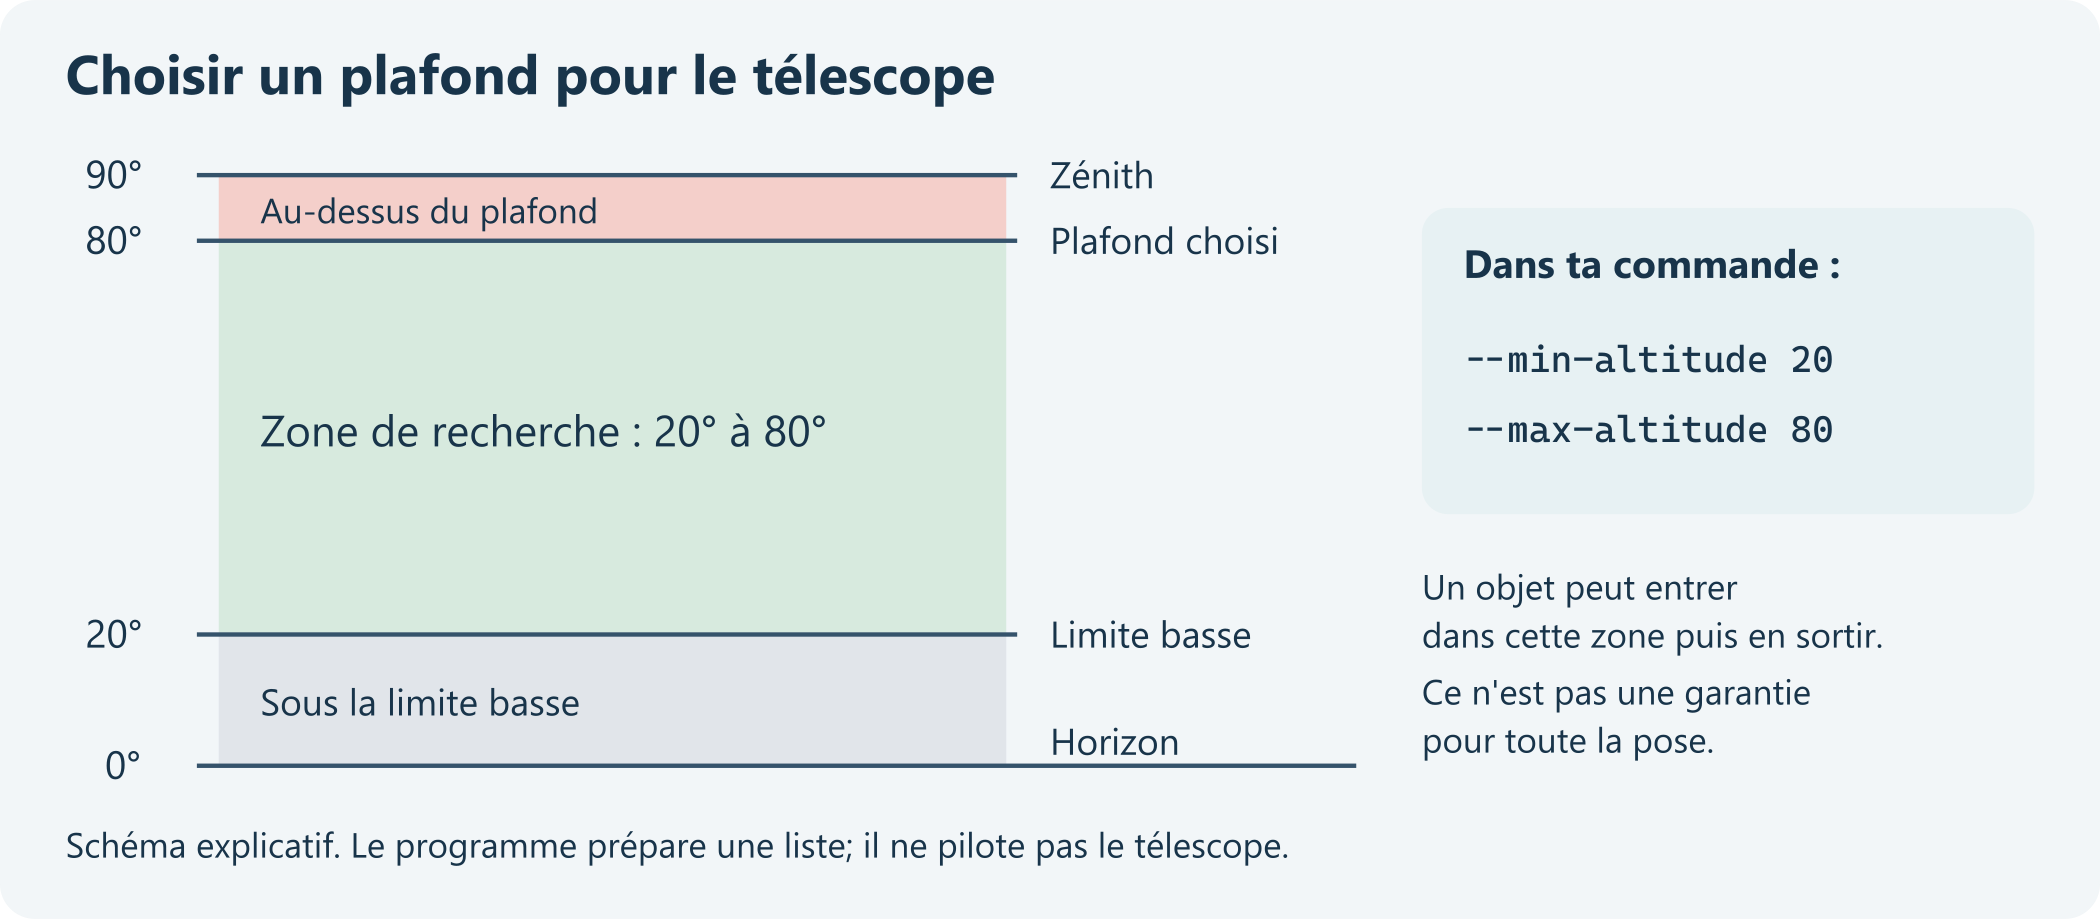
\includegraphics[width=\linewidth,height=28mm,keepaspectratio]{figures/image33.png}\par{\scriptsize Figure 35.1 — Délimitation de la zone d'observation entre 20° et 80° d'altitude (Prud'Homme, 2026b).\par}\end{minipage}\hfill

\begin{minipage}[t]{.48\linewidth}\centering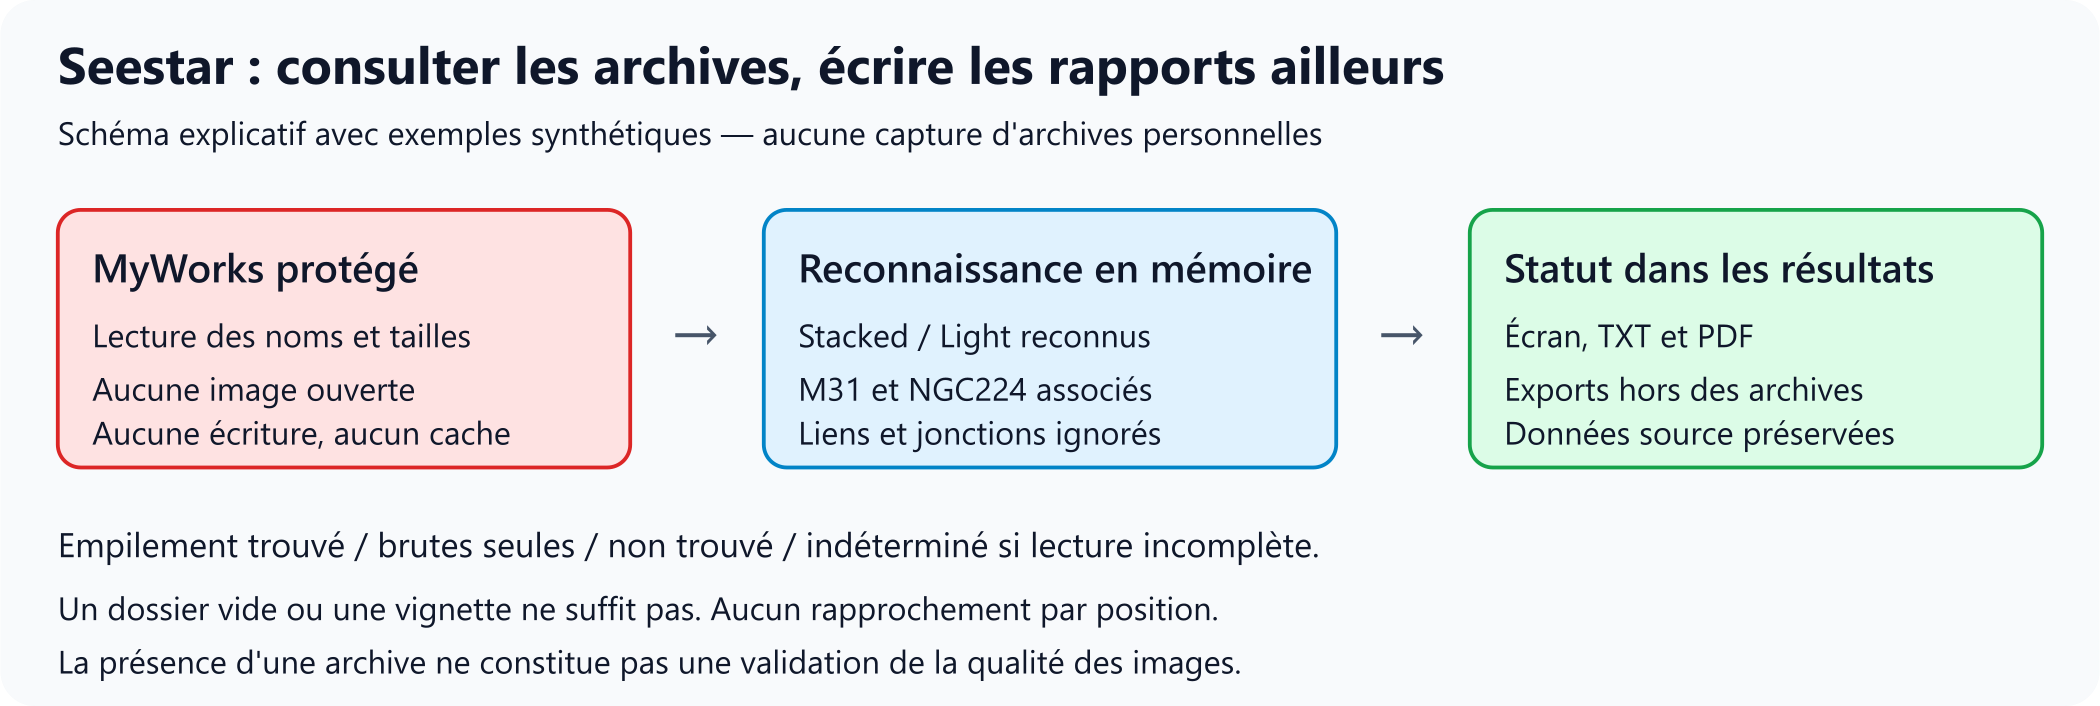
\includegraphics[width=\linewidth,height=28mm,keepaspectratio]{figures/image34.png}\par{\scriptsize Figure 35.2 — Consultation des archives Seestar S50 en mode lecture seule strict (Prud'Homme, 2026b).\par}\end{minipage}\par

\begin{minipage}[t]{.48\linewidth}\centering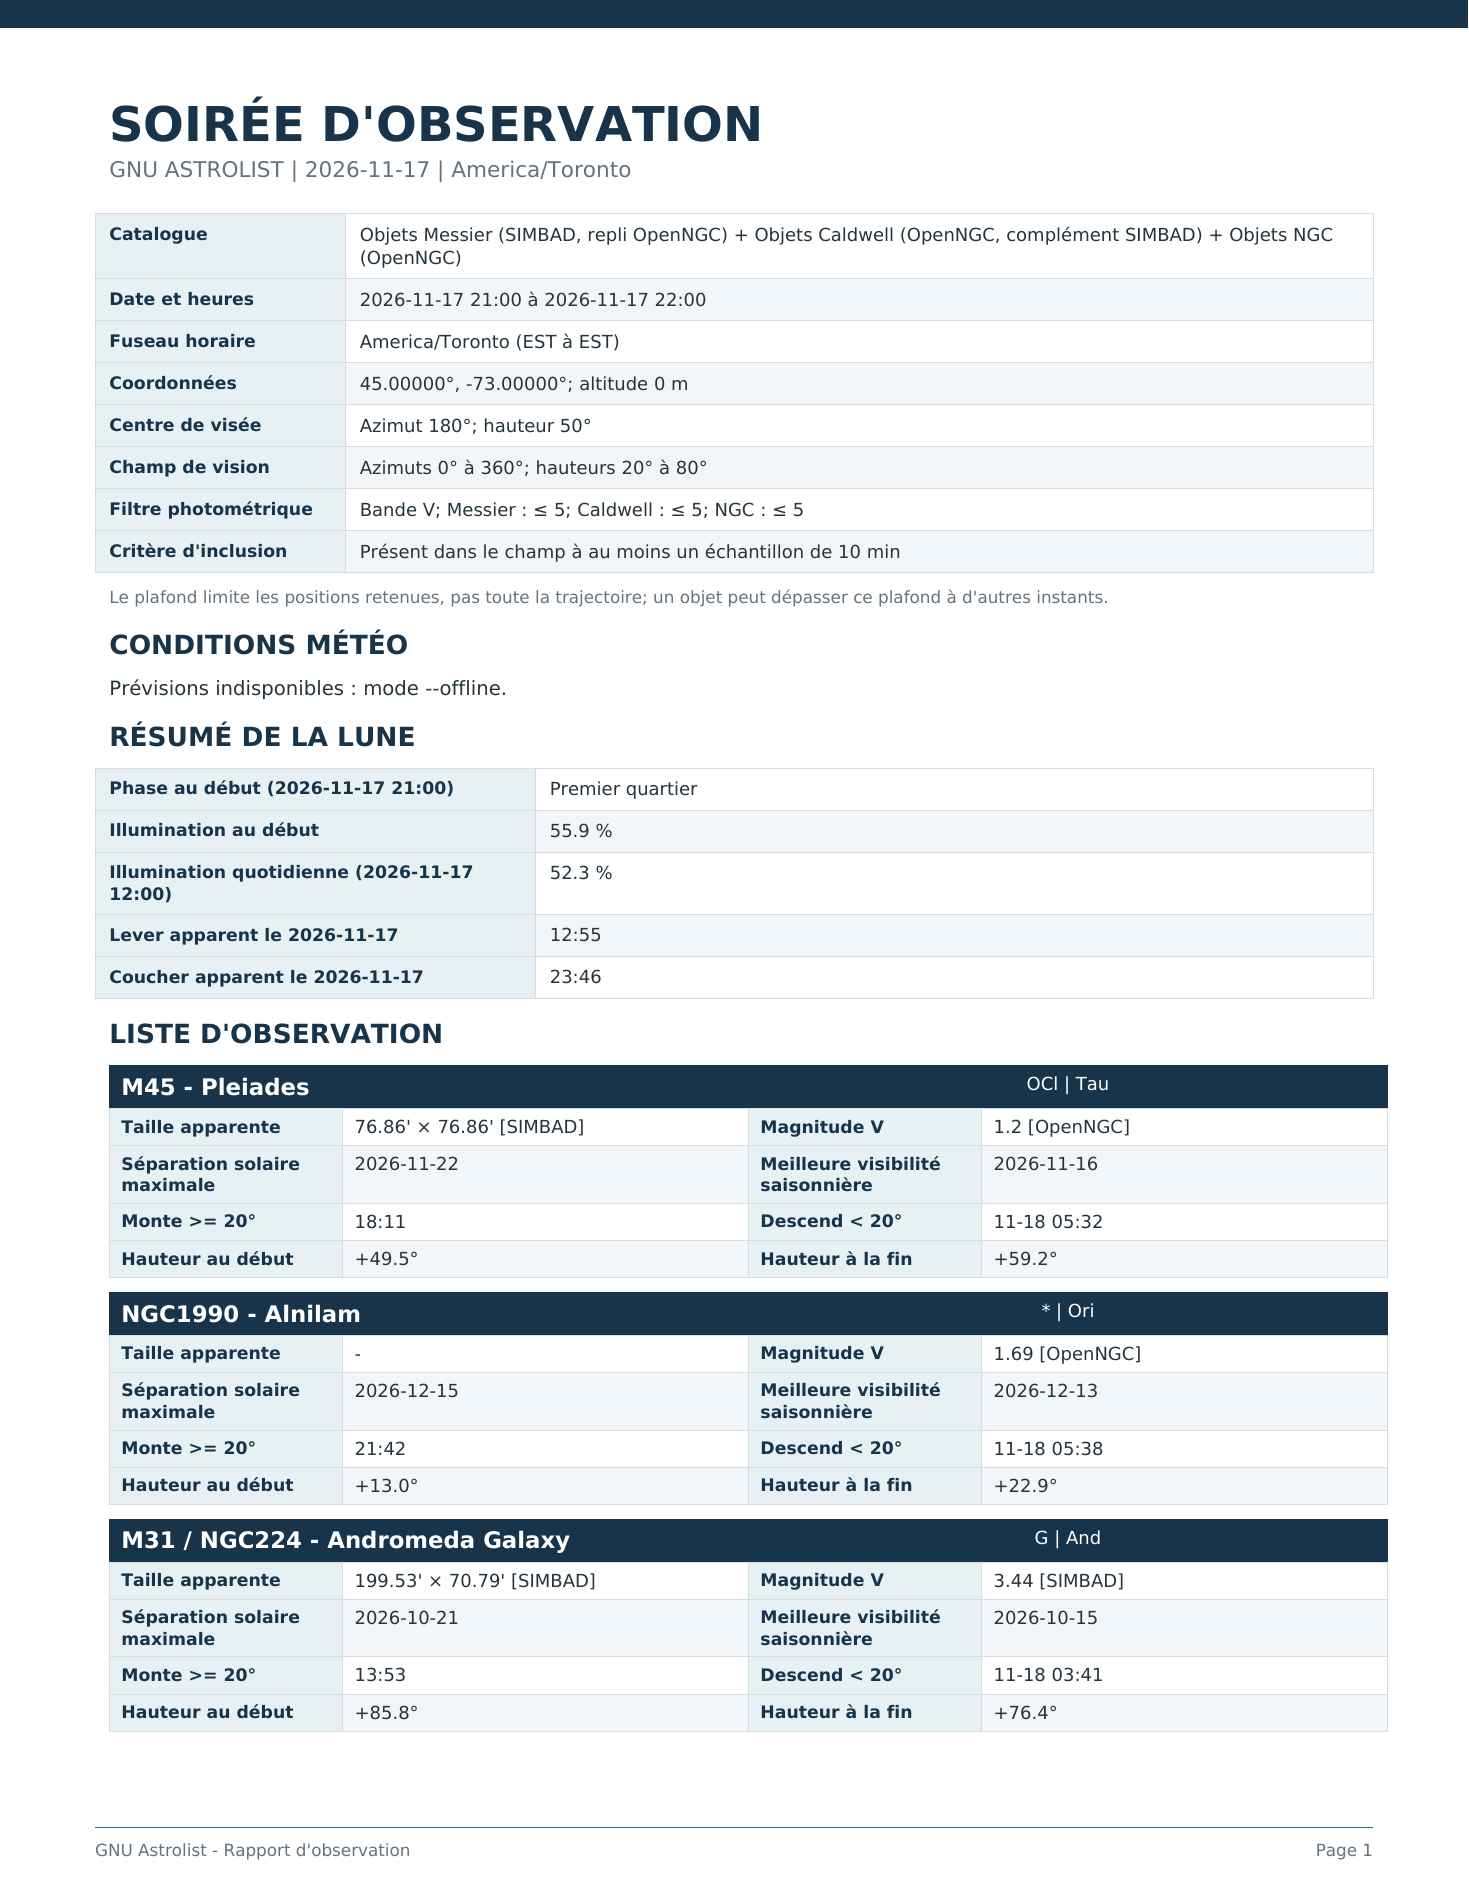
\includegraphics[width=\linewidth,height=28mm,keepaspectratio]{figures/image35.png}\par{\scriptsize Figure 35.3 — Rapport PDF « Soirée d'observation » généré par GNU Astrolist (M45, NGC1990, M31) (Prud'Homme, 2026b).\par}\end{minipage}\hfill

\par\medskip\textbf{À projeter.} Après le rapport antérieur, projetez la commande puis la sortie du calcul du 24 novembre. Commande à saisir sur une seule ligne : \par{\raggedright\ttfamily\small gnu-astrolist -{}-date 2026-11-24 -{}-time-range 20:00-22:00 -{}-timezone America/Toronto -{}-lat 45.57 -{}-lon -73.68 -{}-az-min 15 -{}-az-max 180 -{}-min-altitude 20 -{}-objects messier -{}-limit 5 -{}-offline\par} GNU Astrolist 0.11.0 a trouvé 20 objets et en a affiché cinq. À 20 h, M42 est à 3,9°. Elle atteint 20° vers 21 h 38. Le programme inclut un objet s’il entre dans le champ à au moins un échantillon. Le mode hors ligne utilise des données locales, sans météo. La table de rotation terrestre disponible dépasse sa plage de validité : ces hauteurs arrondies servent à planifier la soirée.\par\medskip
\repere{Texte oral}

Le troisième projet, GNU Astrolist, illustre un autre scénario très fréquent : reprendre un vieux logiciel existant et le faire évoluer avec rigueur grâce à l'alliance entre ChatGPT et Codex (Prud'Homme, 2026b). Avant chaque belle nuit dégagée, nous nous posons tous la même question : « Qu'est-ce que je peux photographier ce soir depuis mon terrain ? » Depuis mon jardin, certains arbres bloquent l'horizon bas sous 20 degrés, et mon télescope alt-azimutal peine au-dessus de 80 degrés près du zénith. De plus, je voulais fusionner les catalogues Messier, Caldwell et NGC sans doublons (M31 et NGC 224 regroupés sur une seule ligne) et vérifier automatiquement si j'avais déjà photographié l'objet sur mon Seestar — tout en imposant une règle de sécurité absolue : toucher au disque du Seestar uniquement en lecture seule (Prud'Homme, 2026b). En travaillant par étapes avec Codex directement sur le dépôt GitHub, nous avons ajouté le calcul des passages de satellites (avec heure locale, azimut et hauteur pour le cadrage), les comètes, les astéroïdes et un mode hors connexion qui fonctionne sous la tente sans Wi-Fi. Surtout, j'ai exigé des preuves de qualité : le projet dispose désormais de 800 tests automatisés qui vérifient à chaque modification que rien n'a été cassé !\par

\smallskip\textbf{Animation proposée.} Faites choisir une hauteur minimale pour un site encombré. Repérez dans le rapport une cible à vérifier.

\clearpage\repere{DIAPOSITIVE 43 / 45 · 1:53:30 – 1:57 · 3,5 min}

{\Large\bfseries Des poses archivées aux passages de satellites\par}
\repere{Texte oral et conduite des six vues}
\textbf{0:00–0:30 · L’archive.} Une traînée dans une pose du Seestar attire mon attention. Comment vérifier si elle correspond au passage d’un satellite connu? Je conserve l’image et ses métadonnées. Je mène l’analyse sur une copie.

\textbf{0:30–1:00 · La démarche.} ChatGPT m’aide à préciser le besoin. Avec Codex, je peux écrire et vérifier les étapes du programme. Sur les seize poses, le détecteur a conservé 935 propositions de lignes. Beaucoup sont des résidus. Une proposition appelle un examen des pixels.

\textbf{1:00–1:30 · Les observations.} Regardez la série de huit poses. Chacune dure dix secondes. Environ cinq minutes séparent deux prises. Pointez la huitième image de la série 3.

\textbf{1:30–2:15 · S03-08.} Montrez d’abord la photo du haut. Où voyez-vous la traînée? Passez à la vue annotée. Une ligne vient de la mesure de l’image. L’autre vient d’une prévision orbitale. Leur proximité rend plausible une association avec STARLINK-1301.

\textbf{2:15–2:45 · S04-01.} La quatrième trace est faible. Le dossier conserve cette incertitude : aucune association n’est retenue pour cette pose.

\textbf{2:45–3:30 · Résultats et limites.} Trois poses donnent trois associations plausibles avec des objets distincts : KUIPER-00116 pour S03-03, STARLINK-1301 pour S03-08 et CENTISPACE-1 S13 pour S04-04. L’écart transversal est la distance angulaire entre la ligne mesurée et la ligne prévue. Les trois médianes sont d’environ 60, 34 et 30 secondes d’arc. Ces valeurs décrivent l’accord géométrique et laissent ouvertes les incertitudes. Aucune identité n’est confirmée. Le journal et le tutoriel permettent de rejouer l’étude, actuellement en pause.

\textit{Document illustré de Steve Prud’Homme, 24 novembre 2026, figures 3, 4, 9, 10 et 11.}

\clearpage\repere{DIAPOSITIVE 44 / 45 · 1:57 – 1:58:30 · 1,5 min}

{\Large\bfseries Que voulez-vous essayer à la prochaine Lune?\par}

\smallskip\hrule\smallskip

{\small\textbf{Repère visuel.} Synthèse visuelle : l'alliance entre l'expertise de l'astronome et la puissance de génération de l'IA.\par}

\begin{minipage}[t]{.86\linewidth}\centering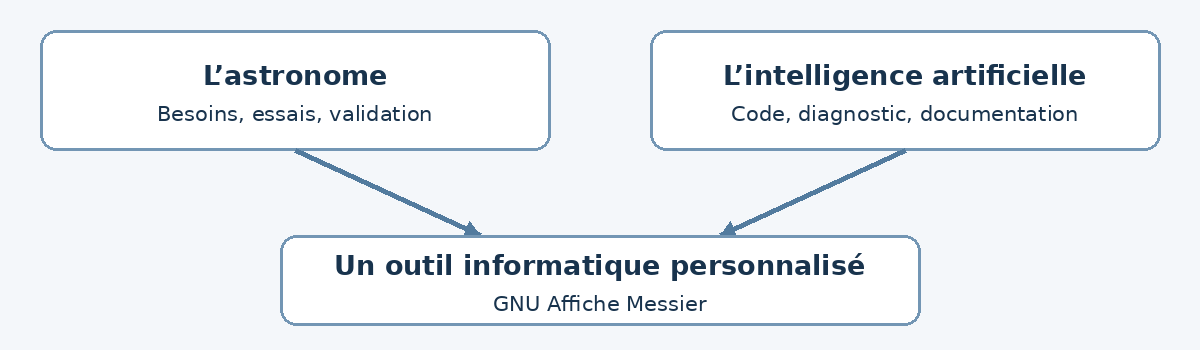
\includegraphics[width=\linewidth,height=40mm,keepaspectratio]{figures/image1.png}\par{\scriptsize Figure 37.1 — L'astronome définit le cap et valide la science ; l'IA accélère la réalisation (Prud'Homme, 2025).\par}\end{minipage}\par

\par\medskip\repere{Texte oral}

Pour conclure ces deux heures ensemble, retenons cette image simple : le Vibe Coding ne remplace pas l'astronome, il démultiplie sa capacité de création (Prud'Homme, 2025 ; Ernaux, 2025). L'intelligence artificielle apporte la maîtrise syntaxique des langages et l'assemblage rapide des bibliothèques, mais c'est vous qui apportez le sens, l'expérience du ciel nocturne, la rigueur des tests et la validation scientifique (Kim et Yegge, 2025 ; Osmani, 2025). N'ayez pas peur de commencer petit : ouvrez une conversation, décrivez un irritant de vos soirées d'observation, sauvegardez vos étapes sur GitHub et partagez vos trouvailles avec le club. Merci beaucoup de votre attention, et bons ciels à toutes et à tous !\par

\smallskip\textbf{Animation proposée.} Accordez trente secondes de réflexion, puis invitez une personne à partager sa tâche et son test.

\clearpage\repere{DIAPOSITIVE 45 / 45 · 1:58:30 – 2:00 · 1,5 min}

{\Large\bfseries Retrouver les projets et les références\par}

\smallskip\hrule\smallskip

{\small\textbf{Repère visuel.} Codes QR d'accès direct aux dépôts GitHub des projets présentés.\par}

\begin{minipage}[t]{.86\linewidth}\centering
\includegraphics[width=\linewidth,height=40mm,keepaspectratio]{figures/image37.png}\par{\scriptsize Figure 38.1 — Codes QR d'accès direct aux dépôts GitHub et à la galerie en ligne (Prud'Homme, 2026a).\par}\end{minipage}\par

\par\medskip\repere{Texte oral}

Vous trouverez dans les diapositives de bibliographie qui suivent, ainsi que dans les notes de la conférence, l'ensemble des références bibliographiques citées ce soir, formatées selon la norme UQAM-APA. Tous mes dépôts de code source, mes schémas et mes guides d'installation sont librement accessibles sur mon compte GitHub (github.com/steveprudhomme). Je suis maintenant à votre disposition pour répondre à vos questions et discuter de vos idées de projets !\par

\clearpage\section*{Références bibliographiques}

\nocite{*}\bibliographystyle{atelier-uqam}\bibliography{references}

\end{document}
